% ------------------------------------------------------------------------
% ------------------------------------------------------------------------
% Modelo UFSC para Trabalhos Academicos (tese de doutorado, dissertação de
% mestrado) utilizando a classe abntex2
%
% Autor: Alisson Lopes Furlani
% 	Modificações:
%	- 27/08/2019: Alisson L. Furlani, add pacote 'glossaries' para listas
%   - 06/11/2019: Luiz-Rafael Santos, modifica para Trabalho de Conclusão de Curso
% ------------------------------------------------------------------------
% ------------------------------------------------------------------------

\documentclass[
	% -- opções da classe memoir --
	12pt,				% tamanho da fonte
	%openright,			% capítulos começam em pág ímpar (insere página vazia caso preciso)
	oneside,			% para impressão no anverso. Oposto a twoside
	a4paper,			% tamanho do papel. 
	% -- opções da classe abntex2 --
	chapter=TITLE,		% títulos de capítulos convertidos em letras maiúsculas
	section=TITLE,		% títulos de seções convertidos em letras maiúsculas
	%subsection=TITLE,	% títulos de subseções convertidos em letras maiúsculas
	%subsubsection=TITLE,% títulos de subsubseções convertidos em letras maiúsculas
	% -- opções do pacote babel --
	english,			% idioma adicional para hifenização
	%french,				% idioma adicional para hifenização
	%spanish,			% idioma adicional para hifenização
	brazil				% o último idioma é o principal do documento
	]{abntex2}

\usepackage{setup/ufscthesisA4-alf}
\usepackage{multirow}
\newcommand{\red}[1]{\textcolor{red}{#1}}

% ---
% Filtering and Mapping Bibliographies
% ---
% Pacotes de citações
% ---
\usepackage{csquotes}
\usepackage[backend = biber, style = abnt]{biblatex}
% FIXME Se desejar estilo numérico de citações,  comente a linha acima e descomente a linha a seguir.
% \usepackage[backend = biber, style = numeric-comp]{biblatex}

\setlength\bibitemsep{\baselineskip}
\DeclareFieldFormat{url}{Disponível~em:\addspace\url{#1}}
\NewBibliographyString{sineloco}
\NewBibliographyString{sinenomine}
\DefineBibliographyStrings{brazil}{%
	sineloco     = {\mkbibemph{S\adddot l\adddot}},
	sinenomine   = {\mkbibemph{s\adddot n\adddot}},
	andothers    = {\mkbibemph{et\addabbrvspace al\adddot}},
	in			 = {\mkbibemph{In:}}
}

\addbibresource{aftertext/references.bib} % Seus arquivos de referências

% ---
\DeclareSourcemap{
	\maps[datatype=bibtex]{
		% remove fields that are always useless
		\map{
			\step[fieldset=abstract, null]
			\step[fieldset=pagetotal, null]
		}
		% remove URLs for types that are primarily printed
%		\map{
%			\pernottype{software}
%			\pernottype{online}
%			\pernottype{report}
%			\pernottype{techreport}
%			\pernottype{standard}
%			\pernottype{manual}
%			\pernottype{misc}
%			\step[fieldset=url, null]
%			\step[fieldset=urldate, null]
%		}
		\map{
			\pertype{inproceedings}
			% remove mostly redundant conference information
			\step[fieldset=venue, null]
			\step[fieldset=eventdate, null]
			\step[fieldset=eventtitle, null]
			% do not show ISBN for proceedings
			\step[fieldset=isbn, null]
			% Citavi bug
			\step[fieldset=volume, null]
		}
	}
}
% ---

% ---
% Informações de dados para CAPA e FOLHA DE ROSTO
% ---
% FIXME Substituir 'Nome completo do autor' pelo seu nome.
\autor{Ramon de Araujo Borba}
% FIXME Substituir 'Título do trabalho' pelo título da trabalho.
\titulo{Plano de testes para módulos de gerenciamento de energia de CubeSats}
% FIXME Substituir 'Subtítulo (se houver)' pelo subtítulo da trabalho.  
% Caso não tenha substítulo, comente a linha a seguir.
% \subtitulo{Subtítulo (se houver)}
% FIXME Substituir 'XXXXXX' pelo nome do seu
% orientador.
\orientador{Prof. Eduardo Augusto Bezerra, Dr.}
% FIXME Se for orientado por uma mulher, comente a linha acima e descomente a linha a seguir.
% \orientador[Orientadora]{Nome da orientadora, Dra.}
% FIXME Substituir 'XXXXXX' pelo nome do seu
% coorientador. Caso não tenha coorientador, comente a linha a seguir.
% \coorientador{Prof. XXXXXX, Dr.}
% FIXME Se for coorientado por uma mulher, comente a linha acima e descomente a linha a seguir.
% \coorientador[Coorientadora]{XXXXXX, Dra.}
% FIXME Substituir 'XXXXXX' pelo nome do Coordenador do 
% programa/curso.
\coordenador{Prof. Fernando Rangel, Dr.}
% FIXME Se for coordenadora mulher, comente a linha acima e descomente a linha a seguir.
% \coordenador[Coordenadora]{Nome da Coordenadora, Dra.}
% FIXME Substituir '[ano da entrega]' pelo ano (ano) em que seu trabalho foi defendido.
\ano{2024}
% FIXME Substituir '[dia] de [mês] de [ano]' pela data em que ocorreu sua defesa.
\data{[dia] de Fevereiro de 2024}
% FIXME Substituir '[Cidade da defesa]' pela cidade em que ocorreu sua defesa.
\local{Florianópolis}
\instituicaosigla{UFSC}
\instituicao{Universidade Federal de Santa Catarina}
% FIXME Substituir 'Dissertação/Tese' pelo tipo de trabalho (Tese, Dissertação). 
\tipotrabalho{Trabalho de Conclusão de Curso}
% FIXME Substituir '[licenciado/bacharel] em [nome do título obtido]' pela grau adequado.
\formacao{bacharel em Engenharia Eletrônica}
% FIXME Substituir '[licenciado/bacharel]' pelo nivel adequado.
\nivel{bacharel}
% FIXME Substituir 'Curso de Graduação em [XXXXXXXX]' pela curso adequado.
\programa{Curso de Graduação em Engenharia Eletrônica}
% FIXME Substituir 'Campus XXXXXX ou Centro de XXXXXX' pelo campus ou centro adequado.
\centro{Centro Tecnológico}
\preambulo
{%
\imprimirtipotrabalho~do~\imprimirprograma~do~\imprimircentro~da~\imprimirinstituicao~para~a~obtenção~do~título~de~\imprimirformacao.
}
% ---

% ---
% Configurações de aparência do PDF final
% ---
% alterando o aspecto da cor azul
\definecolor{blue}{RGB}{41,5,195}
% informações do PDF
\makeatletter
\hypersetup{
     	%pagebackref=true,
		pdftitle={\@title}, 
		pdfauthor={\@author},
    	pdfsubject={\imprimirpreambulo},
	    pdfcreator={LaTeX with abnTeX2},
		pdfkeywords={ufsc, latex, abntex2}, 
		colorlinks=true,       		% false: boxed links; true: colored links
    	linkcolor=black,%blue,          	% color of internal links
    	citecolor=black,%blue,        		% color of links to bibliography
    	filecolor=black,%magenta,      		% color of file links
		urlcolor=black,%blue,
		bookmarksdepth=4
}
\makeatother
% ---

% ---
% compila a lista de abreviaturas e siglas e a lista de símbolos
% ---

% Declaração das siglas
% \siglalista{ABNT}{Associação Brasileira de Normas Técnicas}
\newacronym{OBDH}{OBDH}{On Board Data Handling}
\newacronym{TTC}{TT\&C}{Telemetry Tracking \& Command}
\newacronym{EPS}{EPS}{Electrical Power System}
\newacronym{EPS2}{EPS 2.0}{Electrical Power System 2.0}
\newacronym{REEPS}{RE\(^2\)PS}{Reliability Enchanced Electrical Power System}
\newacronym{ECSS}{ECSS}{European Cooperation for Space Standardization}
\newacronym{ESA}{ESA}{European Space Agency}
\newacronym{DET}{DET}{Direct Energy Transfer}
\newacronym{PPT}{PPT}{Peak Power Transfer}
\newacronym{MPPT}{MPPT}{Maximum Power Point Tracking}
\newacronym{BCR}{BCR}{Battery Charge Regulator}
\newacronym{I2C}{I\(^2\)C}{Inter Integrated Circuit}
\newacronym{COTS}{COTS}{Commercial-off-the-shelf}
\newacronym{AIV}{AIV}{Assembly, Integration and Verification}
\newacronym{UFSC}{UFSC}{Universidade Federal de Santa Catarina}
\newacronym{CDS}{CDS}{Cubesat Design Specification}
\newacronym{PO}{P\&O}{Perturb and Observe}
\newacronym{DoD}{DoD}{Depth of Discharge}
\newacronym{UART}{UART}{Universal Asynchronous Receiver-Transmitter}
\newacronym{PWM}{PWM}{Pulse Width Modulation}


% Declaração dos simbolos
% \simbololista{C}{\ensuremath{C}}{Circunferência de um círculo}
% \simbololista{pi}{\ensuremath{\pi}}{Número pi} 
% \simbololista{r}{\ensuremath{r}}{Raio de um círculo}
% \simbololista{A}{\ensuremath{A}}{Área de um círculo}

% compila a lista de abreviaturas e siglas e a lista de símbolos
\makenoidxglossaries 

% ---

% ---
% compila o indice
% ---
\makeindex
% ---

% ----
% Início do documento
% ----
\begin{document}

% Seleciona o idioma do documento (conforme pacotes do babel)
%\selectlanguage{english}
\selectlanguage{brazil}

% Retira espaço extra obsoleto entre as frases.
\frenchspacing 

% Espaçamento 1.5 entre linhas
\OnehalfSpacing

% Corrige justificação
%\sloppy

% ----------------------------------------------------------
% ELEMENTOS PRÉ-TEXTUAIS
% ----------------------------------------------------------
% \pretextual %a macro \pretextual é acionado automaticamente no início de \begin{document}
% ---
% Capa, folha de rosto, ficha bibliografica, errata, folha de apróvação
% Dedicatória, agradecimentos, epígrafe, resumos, listas
% ---
% ---
% Capa
% ---
\imprimircapa
% ---

% ---
% Folha de rosto
% (o * indica que haverá a ficha bibliográfica)
% ---
\imprimirfolhaderosto*
% ---

% ---
% Inserir a ficha bibliografica
% ---
% http://ficha.bu.ufsc.br/
\begin{fichacatalografica}
	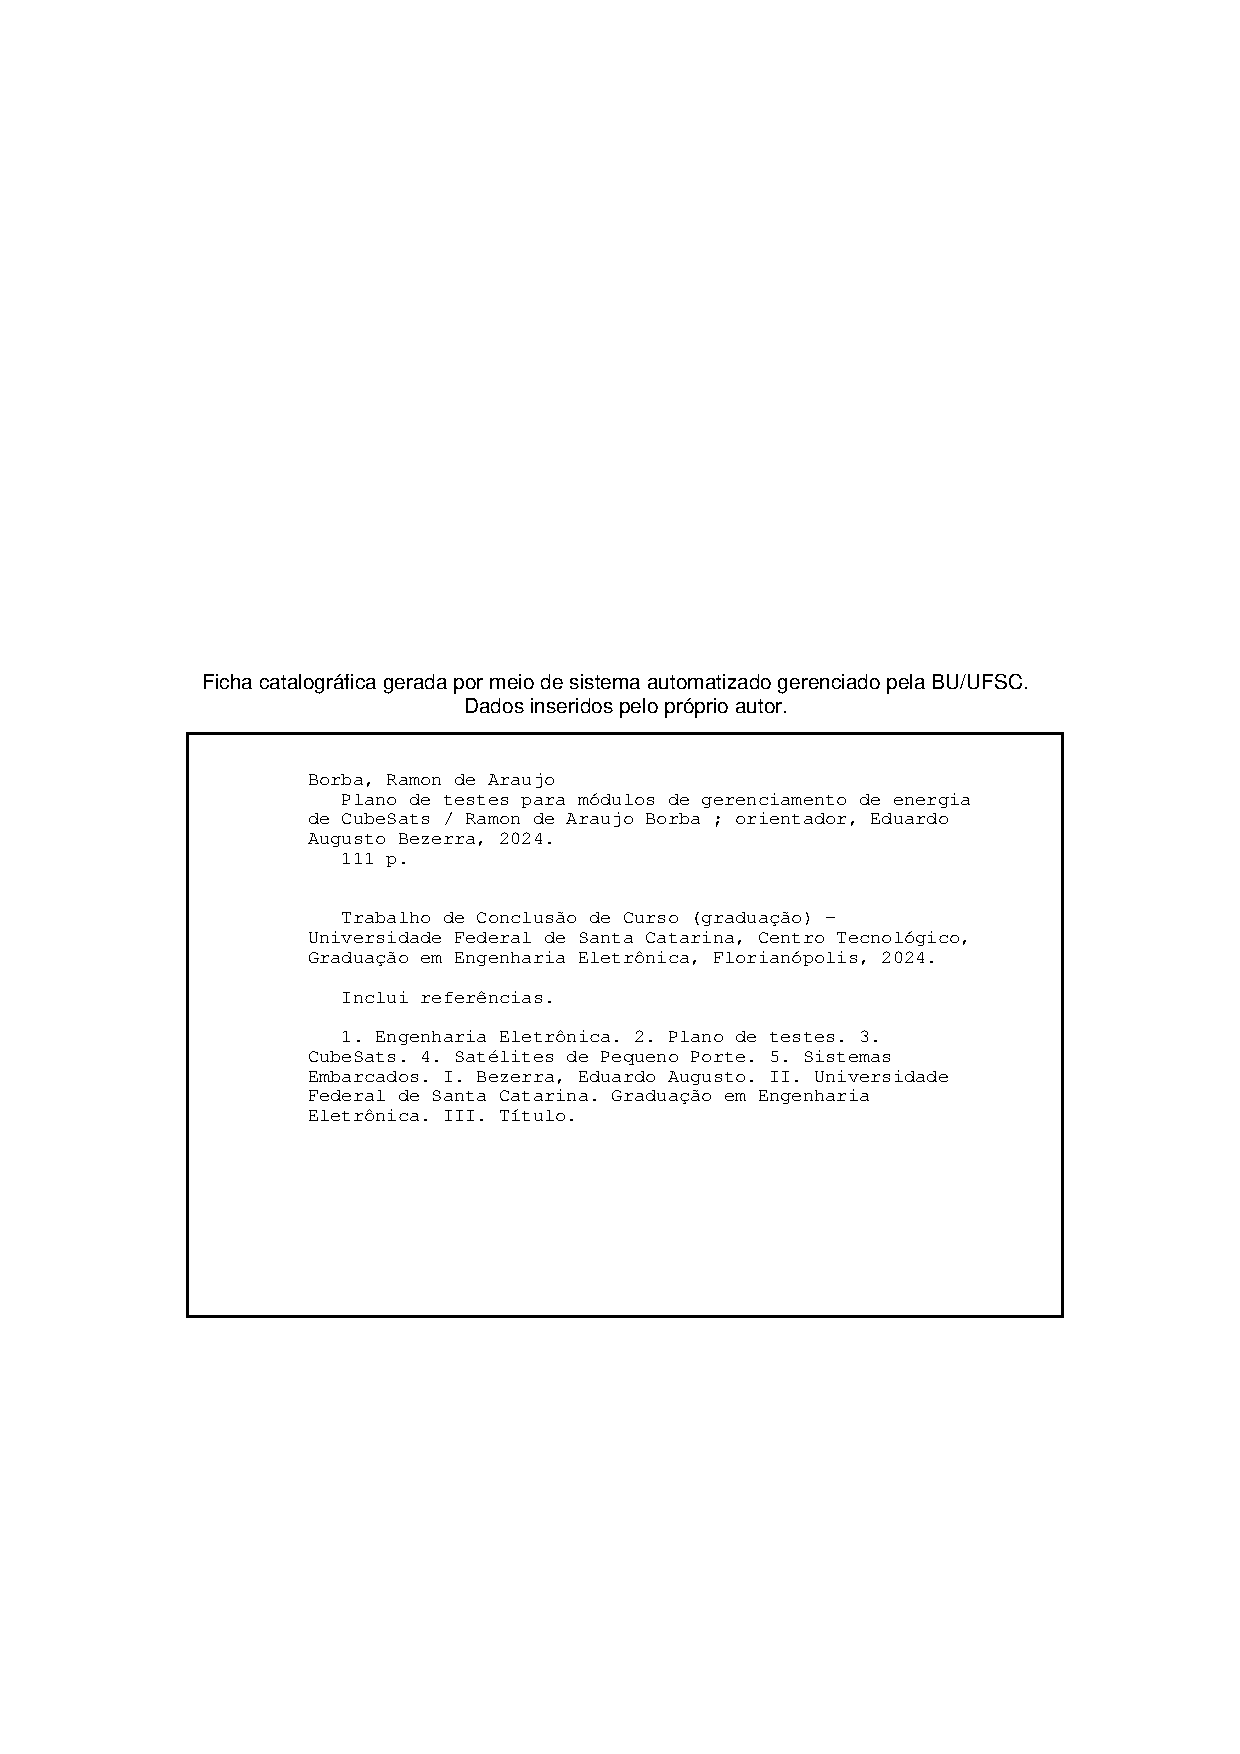
\includepdf{beforetext/Ficha_Catalografica.pdf}
\end{fichacatalografica}
% ---

% ---
% Inserir folha de aprovação
% ---
\begin{folhadeaprovacao}
	\OnehalfSpacing
	\centering
	\imprimirautor\\%
	\vspace*{10pt}		
	\textbf{\imprimirtitulo}%
	\ifnotempty{\imprimirsubtitulo}{:~\imprimirsubtitulo}\\%
	%		\vspace*{31.5pt}%3\baselineskip
	\vspace*{\baselineskip}
	%\begin{minipage}{\textwidth}
	% ~do~\imprimirprograma~do~\imprimircentro~da~\imprimirinstituicao~para~a~obtenção~do~título~de~\imprimirformacao.
	Este~\imprimirtipotrabalho~foi julgado adequado para obtenção do Título de “\imprimirformacao” e aprovado em sua forma final pelo~\imprimirprograma. \\
		\vspace*{\baselineskip}
	\imprimirlocal, \imprimirdata. \\
	\vspace*{2\baselineskip}
	\assinatura{\OnehalfSpacing\imprimircoordenador \\ \imprimircoordenadorRotulo~do Curso}
	\vspace*{2\baselineskip}
	\textbf{Banca Examinadora:} \\
	\vspace*{\baselineskip}
	\assinatura{\OnehalfSpacing\imprimirorientador \\ \imprimirorientadorRotulo}
	%\end{minipage}%
	\vspace*{\baselineskip}
	\assinatura{Prof.(a) xxxx, Dr(a).\\
	Avaliador(a) \\
	Instituição xxxx}

	\vspace*{\baselineskip}
	\assinatura{Prof.(a) xxxx, Dr(a).\\
	Avaliador(a) \\
	Instituição xxxx}


\end{folhadeaprovacao}
% ---

% ---
% Dedicatória
% ---
\begin{dedicatoria}
	\vspace*{\fill}
	\noindent
	\begin{adjustwidth*}{}{5.5cm}     
		Este trabalho é dedicado aos meus colegas de classe e aos meus queridos pais.
	\end{adjustwidth*}
\end{dedicatoria}
% ---

% ---
% Agradecimentos
% ---
\begin{agradecimentos}
	Inserir os agradecimentos aos colaboradores à execução do trabalho. 
	
	Xxxxxxxxxxxxxxxxxxxxxxxxxxxxxxxxxxxxxxxxxxxxxxxxxxxxxxxxxxxxxxxxx. 
\end{agradecimentos}
% ---

% ---
% Epígrafe
% ---
\begin{epigrafe}
	\vspace*{\fill}
	\begin{flushright}
		\textit{``Texto da Epígrafe.\\
			Citação relativa ao tema do trabalho.\\
			É opcional. A epígrafe pode também aparecer\\
			na abertura de cada seção ou capítulo.\\
			Deve ser elaborada de acordo com a NBR 10520.''\\
			(Autor da epígrafe, ano)}
	\end{flushright}
\end{epigrafe}
% ---

% ---
% RESUMOS
% ---

% resumo em português
\setlength{\absparsep}{18pt} % ajusta o espaçamento dos parágrafos do resumo
\begin{resumo}
	\SingleSpacing
	No resumo são ressaltados o objetivo da pesquisa, o método utilizado, as discussões e os resultados com destaque apenas para os pontos principais. O resumo deve ser significativo, composto de uma sequência de frases concisas, afirmativas, e não de uma enumeração de tópicos. Não deve conter citações. Deve usar o verbo na voz ativa e na terceira pessoa do singular. O texto do resumo deve ser digitado, em um único bloco, sem espaço de parágrafo. O espaçamento entre linhas é simples e o tamanho da fonte é 12. Abaixo do resumo, informar as palavras-chave (palavras ou expressões significativas retiradas do texto) ou, termos retirados de thesaurus da área. Deve conter de 150 a 500 palavras. O resumo é elaborado de acordo com a NBR 6028.
	
	\textbf{Palavras-chave}: Palavra-chave 1. Palavra-chave 2. Palavra-chave 3.
\end{resumo}

% resumo em inglês
\begin{resumo}[Abstract]
	\SingleSpacing
	\begin{otherlanguage*}{english}
		Resumo traduzido para outros idiomas, neste caso, inglês. Segue o formato do resumo feito na língua vernácula. As palavras-chave traduzidas, versão em língua estrangeira, são colocadas abaixo do texto precedidas pela expressão “Keywords”, separadas por ponto.
		
		\textbf{Keywords}: Keyword 1. Keyword 2. Keyword 3.
	\end{otherlanguage*}
\end{resumo}

%% resumo em francês 
%\begin{resumo}[Résumé]
% \begin{otherlanguage*}{french}
%    Il s'agit d'un résumé en français.
% 
%   \textbf{Mots-clés}: latex. abntex. publication de textes.
% \end{otherlanguage*}
%\end{resumo}
%
%% resumo em espanhol
%\begin{resumo}[Resumen]
% \begin{otherlanguage*}{spanish}
%   Este es el resumen en español.
%  
%   \textbf{Palabras clave}: latex. abntex. publicación de textos.
% \end{otherlanguage*}
%\end{resumo}
%% ---

{%hidelinks
	\hypersetup{hidelinks}
	% ---
	% inserir lista de ilustrações
	% ---
	\pdfbookmark[0]{\listfigurename}{lof}
	\listoffigures*
	\cleardoublepage
	% ---
	
	% ---
	% inserir lista de quadros
	% ---
	\pdfbookmark[0]{\listofquadrosname}{loq}
	\listofquadros*
	\cleardoublepage
	% ---
	
	% ---
	% inserir lista de tabelas
	% ---
	\pdfbookmark[0]{\listtablename}{lot}
	\listoftables*
	\cleardoublepage
	% ---
	
	% ---
	% inserir lista de abreviaturas e siglas (devem ser declarados no preambulo)
	% ---
	\imprimirlistadesiglas
	% ---
	
	% ---
	% inserir lista de símbolos (devem ser declarados no preambulo)
	% ---
	% \imprimirlistadesimbolos
	% ---
	
	% ---
	% inserir o sumario
	% ---
	\pdfbookmark[0]{\contentsname}{toc}
	\tableofcontents*
	\cleardoublepage
	
}%hidelinks
% ---
% ---

% ----------------------------------------------------------
% ELEMENTOS TEXTUAIS
% ----------------------------------------------------------
\textual

% ---
% Introdução
% ---
% ----------------------------------------------------------
\chapter{Introdução}\label{cap:intro}
% ----------------------------------------------------------

Desde a criação do padrão CubeSat em 1999, nanossatélites tem sido utilizados em cada vez mais aplicações. Popularizado inicialmente no meio acadêmico, possibilitando à universidades o desenvolvimento de missões espaciais de baixo custo, atualmente estes satélites são utilizados para diversas aplicações, como mostrado em \textcite{modern-small-sats-economics}.

Inicialmente os CubeSats serviam um propósito didático, com aplicações de demonstração de tecnologia, experimentos científicos.
Porém, recentemente, aplicações comerciais de nanossatélites e CubeSats tem ganhado espaço, relata \textcite{modern-small-sats-economics} tanto que em 2014 o numero de lançamentos de nanossatélites com propósito comercial ultrapassou os de propósito acadêmico.

Com o advento de conceitos como “\textit{New Space}” e a percepção de sua utilidade comercial, os pequenos satélites estão entrando no radar de grandes empresas, com SpaceX e Boeing, planejando a utilização de grandes constelações, conforme observado por \textcite{modern-small-sats-economics}.
Inclusive, CubeSats vem sendo utilizados em pesquisas e missões espaciais de alto nível, com grandes instituições como a NASA em seu programa Artemis, mostrado em \textcite{artemis-plan}, que utilizará de CubeSats em sua missão com o objetivo de explorar a lua.

% ----------------------------------------------------------
\section{Falhas em CubeSats}\label{sec:intro-falhas}
% ----------------------------------------------------------

Com a proposta de baixo custo, rápido desenvolvimento e uso de componentes \gls{COTS}, a confiabilidade dos CubeSats foi significativamente reduzida em relação à satélites de grande porte, que utilizam componentes robustos desenvolvidos especificamente para aplicações espaciais e passam por processos rigorosos de testes, validação e qualificação.
Como consequência disso, observaram-se grandes taxas de falhas em missões de CubeSats.

Conforme \textcite{survey-nanosat-missions-2010}, até 2010, cerca de 32\% dos lançamentos de nanossatélites resultaram em falha, e considerando apenas os lançamentos bem sucedidos, apenas cerca de 48\% das missões tiveram sucesso total.

O estudo de \textcite{first-100-cubesats}, similarmente aponta taxas de falha de aproximadamente 50\% em missões acadêmicas de CubeSat.
Também neste estudo, esta alta taxa é atribuída a uma carência de testes funcionais a nível de integração dos satélites, visto que, em missões acadêmicas, devido a cronogramas justos ou orçamentos limitados, costuma-se realizar apenas os testes ambientais requeridos para lançamento.
Segundo o autor, estes testes são fundamentais para identificar possíveis falhas na operação do satélite.

No trabalho de \textcite{reliability-of-cubesats}, que analisou a causa de falha de diversos CubeSats lançados até 2014, aponta-se o \gls{EPS} como principal módulo causador de falhas em CubeSats.

Para satélites de propósito educacional, de demonstração tecnológica, essa baixa confiabilidade é tolerável, visto que parte do objetivo destas missões inclui proporcionar experiência e capacitação para estudantes.
Porém, é inaceitável para aplicações comerciais \cite{overview-nanosat-test}.

Esta taxa de falha, no entanto, vem diminuindo desde então, com com uma taxa de apenas 10\% de falhas em lançamentos em 2018 segundo \textcite{aiv-istsat-1}. Conforme a base de dados de nanossatélites Nanosats Database, de \textcite{nanosats-database}, observando a situação dos nanossatélites lançados até dezembro de 2023, mostrados na \autoref{fig:status-nanosats}, tem-se aproximadamente 5\% dos satélites com falhas no lançamento. Ainda, satélites não-operacionais constituem apenas 21\%, aproximadamente, considerando-se os satélites classificados em operacionais ou não-operacionais.
O aumento no número de aplicações comerciais, desenvolvidas por equipes mais experientes e com mais recursos, é um dos fatores que tem contribuído para essa mudança.
Outro fator importante, como relatado em \textcite{aiv-istsat-1}, missões acadêmicas tem dado maior atenção aos processos de \gls{AIV}.

\begin{figure}[htp]
    \caption{Estado atual dos nanossatélites lançados (dezembro de 2023).}
    \begin{center}
        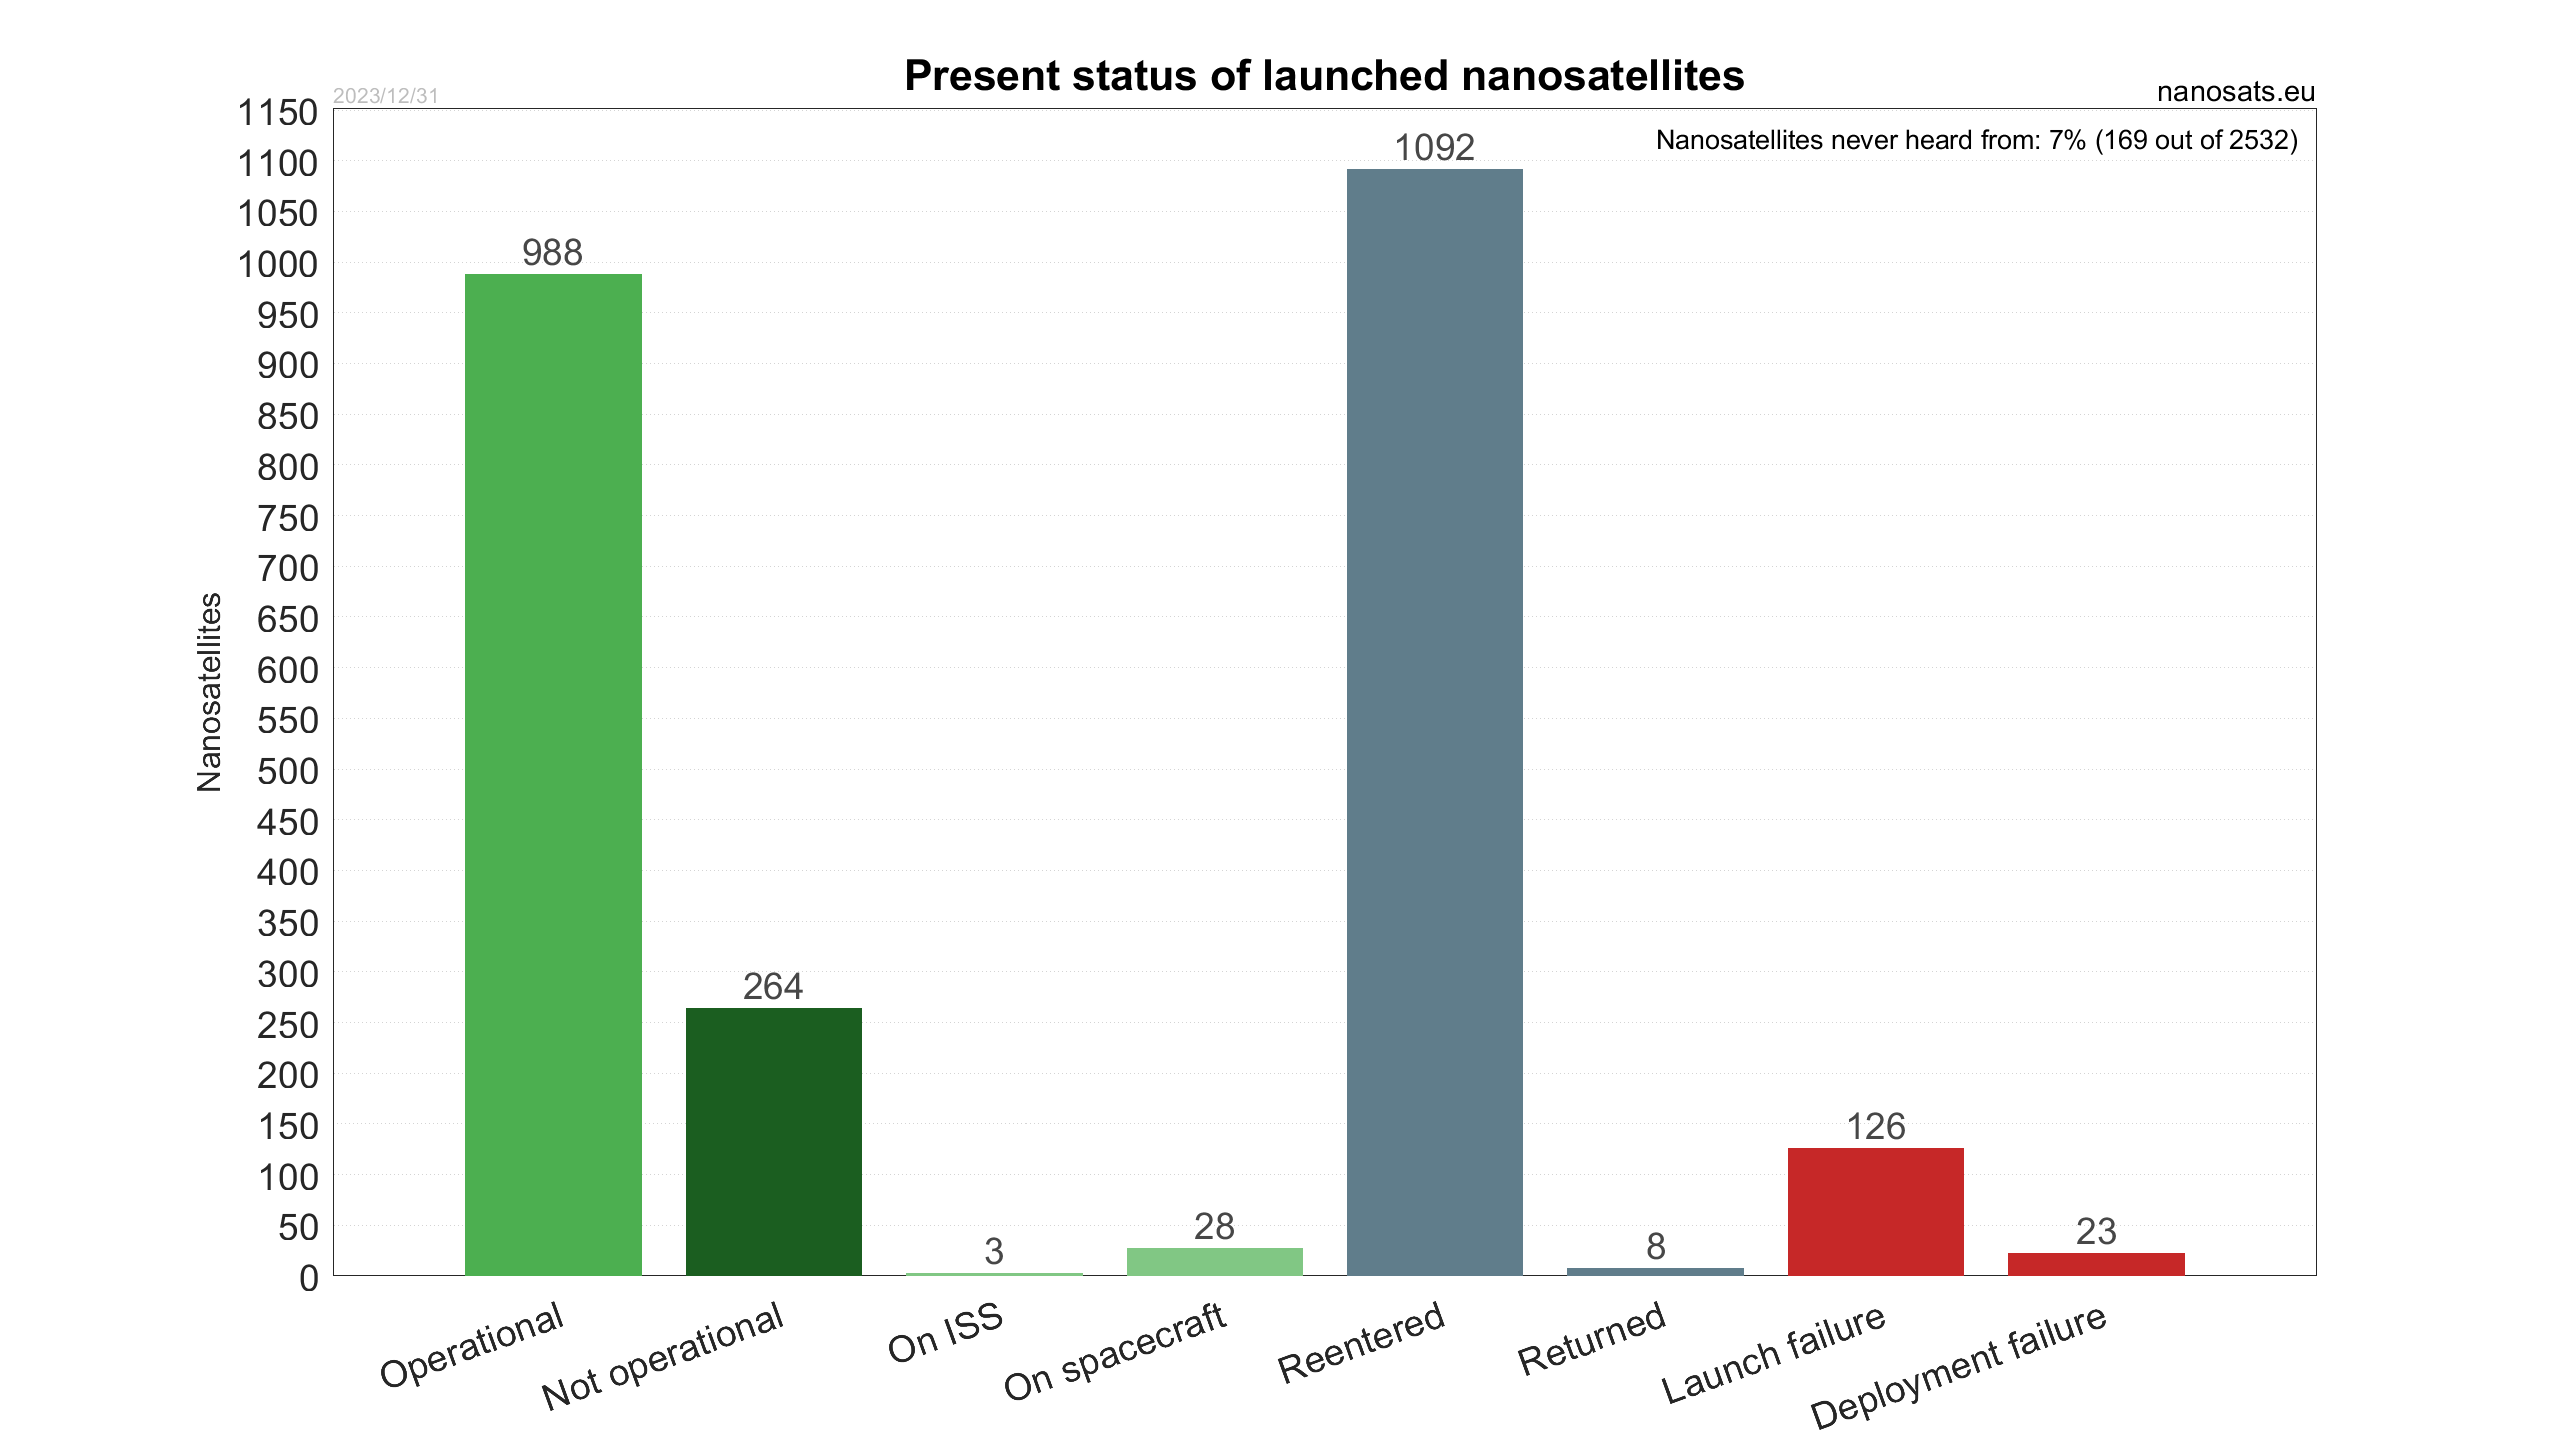
\includegraphics[width=\textwidth, keepaspectratio]{images/Nanosats_status_2023-12-31_large.png}
    \end{center}
    \fonte{\textcite{nanosats-database}.}
    \label{fig:status-nanosats}
\end{figure}


Nota-se também que, em missões de CubeSats mais recentes, foram adotados procedimentos e padrões mais rigorosos, não só em relação à testes, mas em todo o processo de engenharia de sistemas e gerenciamento da missão.
Trabalhos como \textcite{floripasat-1} e \textcite{tailoring-ecss-nanosat}, por exemplo, tomaram como referência os padrões determinados pela \gls{ECSS}, utilizados pela \gls{ESA} e diversas outras agências espaciais da Europa.

% ----------------------------------------------------------
\section{Projetos do SpaceLab}\label{sec:intro-spacelab}
% ----------------------------------------------------------

O FloripaSat-1, descrito em \textcite{floripasat-1}, foi o primeiro CubeSat desenvolvido e lançado pelo Laboratório de Pesquisa em Sistemas Espaciais da UFSC, o SpaceLab, com uma missão de demonstração tecnológica de sua plataforma de serviço multi-missão totalmente desenvolvida por estudantes da \gls{UFSC}.

A plataforma de serviço FloripaSat consiste de três módulos principais, \gls{OBDH}, responsável pelo controle e gerenciamento de dados, \gls{TTC}, responsável pela comunicação com as estações terrestres e recepção de telecomandos, e \gls{EPS}, responsável pela coleta, armazenamento e distribuição de energia.

Após o lançamento do FloripaSat-1, o SpaceLab continuou desenvolvendo e aprimorando sua plataforma de serviço para futuras missões, resultando no desenvolvimento da segunda geração de módulos, que em conjunto formam a plataforma FloripaSat-2 \cite{floripasat2}.

O \gls{EPS2} é a segunda geração de módulo \gls{EPS} desenvolvido para a plataforma multi-missão do laboratório, será utilizado nas missões GOLDS-UFSC e Constelação Catarina e encontra-se nos estágios finais de desenvolvimento. Este \gls{EPS} é uma evolução direta do módulo utilizado no FloripaSat-1, seguindo a mesma arquitetura, porém, aplicando as lições aprendidas com o primeiro lançamento.

Visto que o \gls{EPS} é o principal causador de falhas em CubeSats, iniciou-se também no laboratório a concepção do \gls{REEPS}, com o objetivo de desenvolver um módulo de \gls{EPS} de alta confiabilidade e robustez.

No momento da escrita deste trabalho, o primeiro modelo de engenharia do \gls{REEPS} está em processo de fabricação.
Também, a terceira geração de módulos para a plataforma multi-missão está em fase inicial de desenvolvimento, o que implicará no design de ainda mais um modelo de \gls{EPS} feito no SpaceLab.

Com diferentes projetos, em diferentes estágios de desenvolvimento e diferentes arquiteturas de \gls{EPS} sendo utilizadas nas missões do laboratório, percebeu-se a necessidade de aprimorar os procedimentos de teste utilizados, especialmente na etapa de qualificação, assim como a necessidade de avaliar a performance dos diferentes módulos de \gls{EPS}.

% ----------------------------------------------------------
\section{Motivação}\label{sec:intro-motivacao}
% ----------------------------------------------------------

Como observado anteriormente, processos de \gls{AIV} mais rigorosos, seguindo padrões como \gls{ECSS} adaptados para o cenário de um nanossatélite, tem sido aplicados em missões envolvendo CubeSats, mais especificamente, na etapa de qualificação do satélite como um todo.
Porém, tratando-se dos módulos individualmente, especificamente módulos de EPS, não se observam os mesmos cuidados e estruturação nos procedimentos de teste e a adoção desses padrões, quando mencionados, como em \textcite{mist-eps}, ainda é de forma bastante simplificada.

Neste contexto, propõe-se então a elaboração de um documento contendo diretrizes e orientações acerca da elaboração de planos de testes para módulos \gls{EPS}, baseado nos padrões da \gls{ECSS}, adaptável para diferentes topologias e arquiteturas, a ser utilizado pela equipe do SpaceLab.

Este trabalho consistira na realização de uma revisão de topologias e arquiteturas de EPSs para CubeSats, bem como de campanhas de teste executadas nestes módulos, seguida por uma análise das normas ECSS-E-ST-10-02 \cite{ecss-e-st-10-02} e ECSS-E-ST-10-03 \cite{ecss-e-st-10-03} relacionadas ao processo de verificação e testes. A partir destas analises, será elaborado um documento contento uma série de diretrizes e orientações para a elaboração de planos de testes voltado para EPSs de CubeSats. Por fim, como demonstração, será elaborado um plano de testes simplificado para o \gls{EPS2}, seguindo as orientações propostas.

% ----------------------------------------------------------
\section{Objetivos}\label{sec:objetivos}
% ----------------------------------------------------------

Nas seções abaixo estão descritos o objetivo geral e os objetivos específicos deste trabalho.

% ----------------------------------------------------------
\subsection{Objetivo Geral}
% ----------------------------------------------------------

% Propor uma estrutura de plano de testes aplicável à diferentes topologias de módulos de \gls{EPS}s de CubeSats baseado nos padrões da \gls{ECSS}.

Elaboração de um documento contendo diretrizes e orientações para preparação de planos de teste para módulos \gls{EPS}, baseado nas normas e padrões da \gls{ECSS}, de forma que o mesmo seja aplicável à diferentes topologias e arquiteturas.

% ----------------------------------------------------------
\subsection{Objetivos Específicos}
% ----------------------------------------------------------

\begin{itemize}
    \item Analisar as normas da ECSS relacionadas a procedimentos de teste.
    \item Identificar os principais blocos de teste necessários.
    \item Identificar as principais funções e características de um \gls{EPS} a serem testadas.
    \item Propor uma estrutura de documentação para os testes.
    \item Desenvolver um plano de testes para o \gls{EPS2} baseado na proposta deste trabalho.
\end{itemize}
% ---

% ---
% Funcamentação
% ---
% ----------------------------------------------------------
\chapter{Fundamentação}\label{cap:fundamentacao}
% ----------------------------------------------------------

% ----------------------------------------------------------
\section{O Padrão CubeSat}\label{sec:cubesats}
% ----------------------------------------------------------

Os CubeSats são nano satélites padronizados, com critérios de tamanho, forma e peso específicos.
Satélites neste padrão são compostos por uma ou mais unidades em formato cúbico, com aresta de \(10cm\) e massa de até \(2kg\) \cite{cds}.
Cada unidade é chamada "1U", ou seja, um CubeSat formado por três unidades é categorizado com um CubeSat 3U.

Este padrão surgiu, em 1999, de um projeto colaborativo entre os professores Bob Twiggs (Stanford University) e Jordi Puig-Suari (California Polytechnic State University), chamado CubeSat Project, que tinha como objetivo promover o acesso ao ambiente espacial através da redução de custos e de tempo de desenvolvimento, possibilitando lançamentos mais frequentes \cite{cds}.

Pode-se identificar um conjunto de subsistemas fundamentais presentes no design de boa parte dos 
CubeSats. Nos trabalhos de \textcite{tailoring-ecss-nanosat},- \textcite{survey-nanosat-missions-2010} e \textcite{reliability-of-cubesats} foram identificados os seguintes principais subsistemas:
\begin{alineas}
    \item gerenciamento de energia;
    \item gerenciamento de dados (computador de bordo);
    \item comunicação;
    \item determinação e controle de atitude e orbita;
    \item estrutura mecânica;
    \item controle térmico;
    \item propulsão.
\end{alineas}

Cada subsistema é geralmente implementado em um módulo dedicado, chamado módulo de serviço, e o conjunto destes módulos forma a plataforma de serviço do satélite, responsável por todas as funções e operações fundamentais de um CubeSat.
De fato,  no livro de \textcite{cappelletti_2020}, são apresentados tais módulos e discutidos os principais aspectos a serem considerados para o design e implementação de cada subsistema.

Além da plataforma de serviço, os CubeSats também são equipados com cargas úteis, ou payloads, que são os módulos responsáveis por realizar os objetivos específicos de cada missão.

% ----------------------------------------------------------
\section{Normas e Padrões de Testes}\label{sec:normas-ecss}
% ----------------------------------------------------------
% TODO: Pensar num nome melhor para esta parte

A principal referência a ser seguida em uma missão envolvendo CubeSats é o CubeSat Design Specification, ou \gls{CDS} \cite{cds}, que é o documento que define as especificações do padrão CubeSat.

Além do \gls{CDS}, recentemente, tem-se exemplos de missões de CubeSat seguindo os padrões e normas da \gls{ECSS}, como \textcite{floripasat-1}, \textcite{tailoring-ecss-nanosat} e \textcite{mist-eps}, tanto para etapa de testes quanto para desenvolvimento da missão como um todo.

Ambas estas referências introduzem conceitos e requisitos relevantes à elaboração de um plano de testes que serão apresentados a seguir.

% ==== CubeSat Design Specification ====
\subsection{CubeSat Design Specification}

O \gls{CDS} é um documento contendo as especificações e requisitos básicos e servindo como ponto de partida para o design de CubeSats de 1U a 12U, mantido pela California Polytechnic State University.
Requisitos gerais, mecânicos, elétricos, de operação e de testes são especificados, definindo as características básicas que constituem um nano satélite da classe CubeSat.

Os requisitos de testes descritos no \gls{CDS} estão focados em testes ambientais para o CubeSat como um todo, já em estagio de qualificação para o lançamento.
Como filosofia de testes, o \gls{CDS} propõe as seguintes etapas: \textit{qualification}, \textit{acceptance} e \textit{proto-flight}, executadas conforme o diagrama mostrado na \autoref{fig:test-flow-cds}.

% Fluxograma de testes do CDS
\begin{figure}[htp]
    \caption{Fluxo de testes geral de um CubeSat}
    \begin{center}
        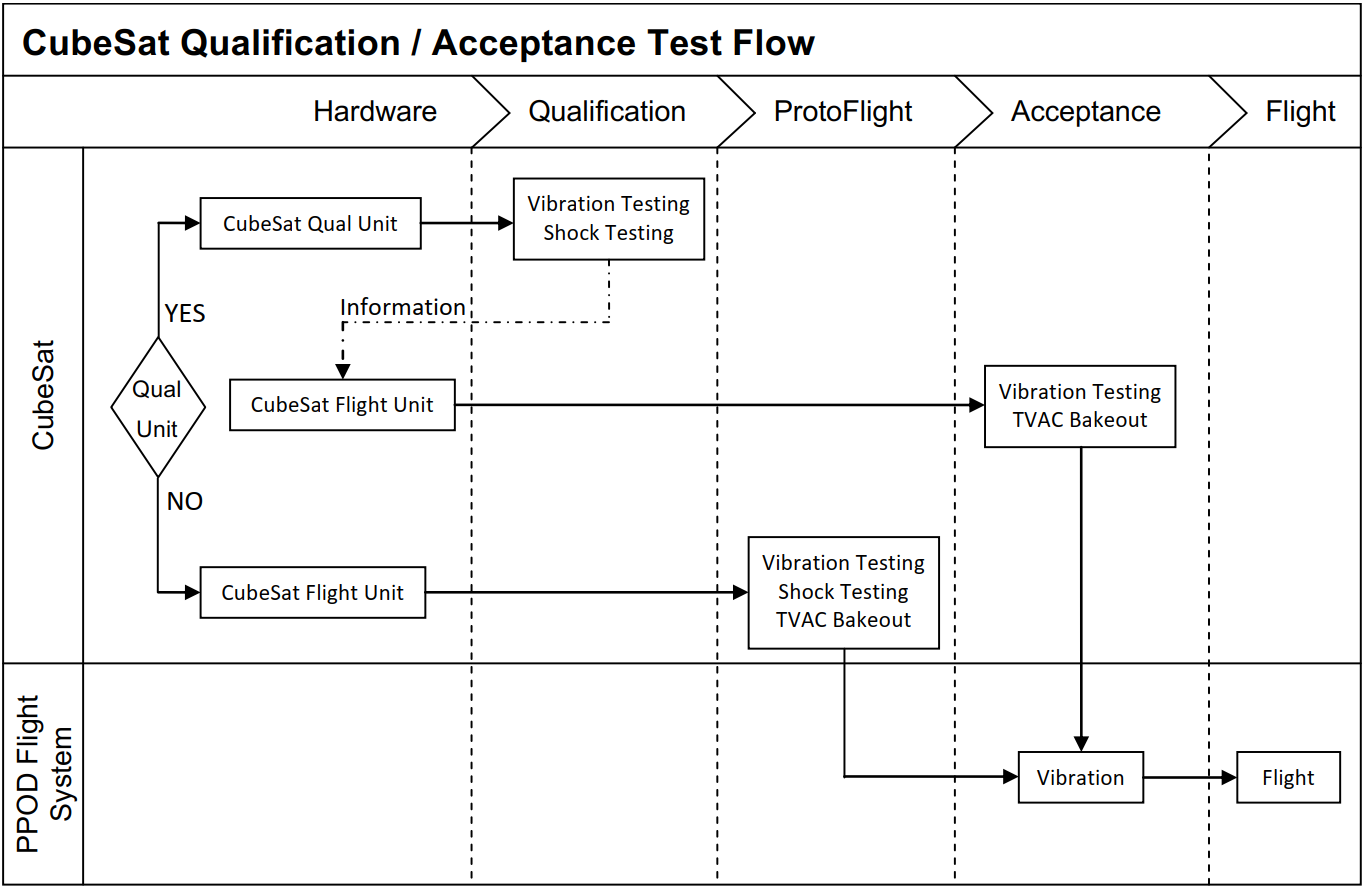
\includegraphics[width=\textwidth, keepaspectratio]{images/test-flow-diagram-cds.png}
    \end{center}
    \fonte{\textcite{cds}.}
    \label{fig:test-flow-cds}
\end{figure}

Os principais testes indicados pelo \gls{CDS} são:
\begin{alineas}
    \item Testes de vibração;
    \item Termo vácuo e bakeout;
    \item Testes de choque;
    \item Inspeção visual;
\end{alineas}

É importante ressaltar que estes requisitos de teste, bem como os parâmetros (intensidade, duração, etc...) de cada teste para cada etapa, como enfatizado no próprio documento, são apenas preliminares e servem somente como base. Os requisitos de teste oficiais para lançamento serão gerados pelo provedor do lançamento, e sempre tomarão precedência em relação aos requisitos do \gls{CDS} ou a qualquer outro conjunto de requisitos.


% ==== European Cooperation For Space Standardization ====
\subsection{European Cooperation for Space Standardization}

A European Cooperation for Space Standardization, ou \gls{ECSS}, é uma colaboração entre a \gls{ESA}, a indústria espacial europeia e diversas outras agências espaciais, responsável por desenvolver e manter um conjunto de normas e padrões relacionados a atividades espaciais. Essas normas e padrões cobrem diversas disciplinas, como gerenciamento, engenharia, controle de qualidade e sustentabilidade.

Dentro do ramo de engenharia, tem-se os documentos ECSS-E-ST-10-02 \cite{ecss-e-st-10-02}, ECSS-E-HB-10-02 \cite{ecss-e-hb-10-02}, ECSS-E-ST-10-03 \cite{ecss-e-st-10-03} e ECSS-E-HB-10-03 \cite{ecss-e-hb-10-03}, que determinam requisitos para os processos de verificação e testes. Estes documentos são redigidos de forma abrangente, com o objetivo de que, a partir de um processo de tailoring, possa-se aplicar estas normas e padrões em diversos níveis, tanto ao satélite completo quanto a um módulo isoladamente.
Como complemento às normas ECSS-E-ST-10-02 e ECSS-E-ST-10-03, tem-se também o documento ECSS-S-ST-00-01 \cite{ecss-s-st-00-01}, um glossário onde diversos termos e definições utilizados nas demais normas são apresentados.
Vale ressaltar também que estes documentos não são específicos para nano satélites, mas foram pensados para satélites de médio e grande porte, onde se necessita uma rigorosidade extrema nos processos de \gls{AIV}.
Portanto deve-se levar em consideração o cenário de uma missão de CubeSat e fazer as adaptações necessárias ao se aplicar estas normas, especialmente em uma missão universitária, visando simplicidade, baixo custo e rápido desenvolvimento.

De acordo com as normas citadas acima, testes são considerados como um dos métodos utilizados para o processo de verificação.
Com isso, apesar deste trabalho ser focado em testes, alguns conceitos relacionados ao processo de verificação, introduzidos em \cite{ecss-e-st-10-02}, como \textit{verification levels}, \textit{verification stages} e \textit{model philosophy}, influenciam diretamente nos objetivos e na elaboração do plano de testes.

Similarmente à filosofia de testes apresentada pelo \gls{CDS}, em \textcite{ecss-e-st-10-03} tem-se os conceitos de \textit{qualification testing}, \textit{acceptance testing} e \textit{proto-flight testing}, que determinam os objetivos do plano de testes.

A seguir são apresentados estes conceitos:

\begin{alineas}
    \item \textit{verification levels}:
    \begin{alineas}
        \item os níveis de verificação estão relacionados à decomposição do produto final, neste caso um CubeSat. estes níveis podem varias de acordo com a complexidade do projeto.
        \item o processo de verificação é executado em cada um dos níveis definidos para um projeto ou missão.
    \end{alineas}

    \item \textit{verification stages}:
    \begin{alineas}
        \item o processo de verificação é feito em estágios, com objetivos específicos. os principais estágios apresentados em \textcite{ecss-e-st-10-02} são \textit{qualification}, \textit{acceptance}\red{, \textit{pre-launch}, \textit{in-orbit}, e \textit{post-landing}}.

        \item o estágio de \textit{qualification} visa garantir que o design proposto para a missão é capaz de cumprir com os requisitos no ambiente esperado.
        \item o estágio de \textit{acceptance} visa demostrar que o modelo final \red{modelo físico de vôo} está em conformidade com o design qualificado previamente
    \end{alineas}

    \item \textit{model philosophy}:
    \begin{alineas}
        \item o conceito de \textit{model philosophy} está relacionado ao tipo e quantidade de modelos físicos utilizados durante o desenvolvimento, verificação e testes.
        \item em \cite{ecss-e-hb-10-02}, diversos tipos de modelos são apresentados e descritos. considerando uma missão de CubeSat, os principais modelos aplicáveis são: modelo de engenharia, modelo de qualificação, modelo de proto-flight e modelo de voo.
    \end{alineas}

    \item \textit{qualification testing}:
    \begin{alineas}
        \item testes de qualificação (chamado \textit{qualification testing} na ECSS-E-ST-10-03) tem o objetivo de verificar que o design do objeto sobre teste é capaz de satisfazer todos os seu requisitos. Estes testes são conduzidos em modelos de qualificação dedicados e com parâmetros de teste (intensidade, duração) específicos.
    \end{alineas}

    \item \textit{acceptance testing}:
    \begin{alineas}
        \item testes de aceitação (chamado \textit{acceptance testing} na ECSS-E-ST-10-03) tem o objetivo de verificar que o objeto sobre teste está em conformidade com o design que foi qualificado previamente e se encontra livre de defeitos de fabricação. Estes testes são conduzidos em todos os modelos de voo e com parâmetros de teste (intensidade, duração) específicos para \textit{acceptance testing}.
    \end{alineas}

    \item \textit{proto-flight testing}:
    \begin{alineas}
        \item testes proto-flight (chamado \textit{proto-flight testing} na ECSS-E-ST-10-03) podem ser executados no primeiro modelo de voo e combinam os objetivos dos testes de qualificação e aceitação. Os parâmetros de teste (intensidade, duração) utilizam as intensidades definidas para qualificação com as durações definidas para aceitação.
    \end{alineas}
\end{alineas}



% ----------------------------------------------------------
\section{Topologias e arquiteturas de EPS}\label{sec:arq-top}
% ----------------------------------------------------------

Nesta seção serão apresentadas diferentes topologias e arquiteturas de \gls{EPS} para CubeSats com o intuito de identificar os principais aspectos e características relevantes para a criação de um plano de testes.

Neste trabalho, topologia se refere a uma visão de alto-nível dos principais blocos funcionais do sistema e arquitetura se refere ao modo como uma dada topologia é implementada.

% ----------------------------------------------------------
\subsection{Topologias}\label{sec:topologias}
% ----------------------------------------------------------

Um módulo \gls{EPS} é composto por algum elementos básicos, mostrados na \autoref{fig:diagrama-basico-eps}.
O sistema de harvesting é responsável por extrair energia dos painéis solares, que são a fonte primaria de energia dos CubeSats.
O sistema de armazenamento de energia é utilizado para alimentar o satélite em períodos de eclipse ou em situações de alta demanda de energia.
O sistema de distribuição é responsável por entregar a energia coletada e armazenada pelo \gls{EPS} de forma adequada às cargas.
Cargas típicas de um \gls{EPS} envolvem os demais subsistemas do satélite, desde de módulos de serviço, como \gls{OBDH} e \gls{TTC}, quanto cargas úteis que variam conforme os objetivos de cada missão.
O barramento que interliga estes elementos, no contexto deste trabalho, será chamado de barramento principal.

\begin{figure}[htp]
    \caption{Diagrama de blocos básico de um \gls{EPS}}
    \begin{center}
        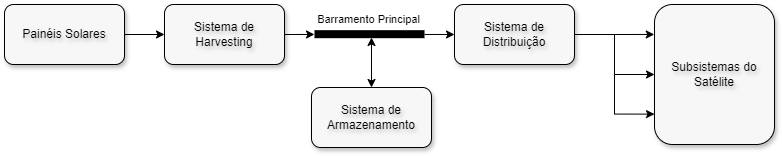
\includegraphics[width=\textwidth, keepaspectratio]{images/basic-eps-block-diagram.png}
    \end{center}
    \fonte{Elaborado pelo autor.}
    \label{fig:diagrama-basico-eps}
\end{figure}


O estudo de \textcite{comprehensive-review-eps} mostra uma revisão de diferentes topologias de \gls{EPS} utilizados em diversas missões e propõe uma forma de classifica-los de acordo com quatro aspectos principais em comum nas diversas topologias:
\begin{alineas}
    \item Estágios de conversão;
    \item Tipo de distribuição; % Localização dos conversores dos barramentos de saída
    \item Tipo de sistema de harvesting;% Sistema de harvesting
    \item Regulação do barramento principal;% Nome melhor para este barramento
\end{alineas}

Estágios de conversão refere-se à quantidade de conversões de energia realizadas até que a energia dos painéis ou baterias seja entregue às cargas. Até o momento, encontram-se em publicações ou patentes apenas topologias com múltiplos estágios de conversão para \gls{EPS}s de CubeSats \cite{comprehensive-review-eps}.

Em relação à localização dos conversores dos barramentos de saída, tem-se topologias centralizadas, com os conversores localizados num mesmo local ou na mesma PCB, ou distribuída, com os conversores localizados em diferentes locais ou PCB com o intuito de estarem fisicamente mais próximos às cargas.

Em relação ao tipo de sistema de harvesting, que realiza a interface com os painéis solares, tem-se topologias com \gls{DET}, onde os painéis são conectados diretamente ao sistema de armazenamento e/ou aos reguladores das cargas, ou topologias com \gls{PPT}, onde os painéis são conectados à conversores dc-dc operados de forma a realizar \gls{MPPT}.
Adicionalmente, no estudo de \textcite{sara-review-eps}, diferenciam-se entre utilização de conversores discretos ou via circuitos integrados, e também apresenta-se a utilização de reguladores VLDO para a interface com os painéis solares.

Em relação à regulação do barramento principal, tem-se topologias com barramento principal regulado, onde há um conversor regulando o mesmo para uma tensão de referência, não-regulado, onde os terminais da bateria são conectados diretamente ao barramento, ou parcialmente regulado, em que o barramento é regulado apenas durante o período iluminado da orbita.



% ----------------------------------------------------------
\subsection{Arquiteturas}\label{sec:arquiteturas}
% ----------------------------------------------------------

A seguir serão analisadas as arquiteturas de diferentes modelos de \gls{EPS}, tanto de desenvolvimento próprio quanto modelos comerciais, a fim de identificar aspectos e características em comum relevantes para o desenvolvimento do plano de testes.

%  ==== Aalto-2 EPS ====
\subsubsection{Aalto-2 EPS}

O \gls{EPS} desenvolvido para o satélite Aalto-2, descrito em \textcite{aalto-eps}, utiliza uma topologia de distribuição centralizada, conversão multe estágio, sistema de harvesting com \gls{PPT} e barramento principal não regulado.
Além disso, possui um microcontrolador MSP430 para controle e monitoramento e redundâncias em hardware para as funcionalidades principais como conversores DC-DC, reguladores de carga de bateria e \gls{MPPT}.

O sistema de harvesting deste \gls{EPS} possui dois canais com CIs dedicados para a realização de \gls{MPPT}. O conjunto de painéis solares de cada eixo, X e Y, é ligado ao barramento principal através de um \gls{BCR}, neste caso o LT3652.

Para armazenamento de energia o EPS do Aalto-2 utilizará duas células de baterias em paralelo (configuração 1s2p). O modelo das baterias ainda não havia sido determinado, porém a inclusão de circuitos de proteção contra over-charge e over-discharge, assim como a necessidade de um sistema de aquecimento para as baterias já estavam previstos.

O sistema de distribuição consiste em dois barramentos, de 3.3V e 5V, utilizando os reguladores LTC1875 e LTC3122 respectivamente.
Cada barramento possui reguladores duplicados em redundância fria.
Possui também um barramento dedicado para alimentar o microcontrolador.
Para controle dos barramentos foram utilizados MOSFETs MAX890L, que além de atuarem como chaves, possuem limitação de corrente proporcionando proteção contra over-current.
Além disso, corrente e tensão nos barramentos são monitoradas pelo microcontrolador.

Para controle e monitoramento, foi utilizado o microcontrolador MSP430-F1611. Tensões, correntes e temperaturas são medidas através do CI LTC2991. Os seguintes dados de telemetria são monitorados e transmitidos ao computador de bordo pelo EPS:
\begin{alineas}
    \item Tensões, correntes e temperaturas dos painéis solares.
    \item Tensões, correntes e temperaturas de cada célula das baterias.
    \item Status de carga das baterias.
    \item Tensões e correntes nos barramentos de saída do EPS.
\end{alineas}


%  ==== ESTCube-1 EPS ====
\subsubsection{ESTCube-1}

O \gls{EPS} desenvolvido para o satélite ESTCube-1, descrito em \textcite{estcube-eps}, utiliza uma topologia de distribuição centralizada, conversão multe estágio, sistema de harvesting com \gls{PPT} e barramento principal não regulado.
Possui também um microcontrolador para controle e monitoramento e inclui redundâncias em hardware.

O sistema de harvesting é composto por três canais de \gls{MPPT}. Cada canal utiliza um chip SPV1040 para a realizar o \gls{MPPT} de um conjunto de painéis correspondente a um dos eixos do satélite.

Duas células de bateria de íon de lítio são utilizadas para armazenamento, com monitoramento de tensão, corrente e temperatura. Cada célula é conectada ao barramento principal através de duas chaves de potência TPS2557, controlando as direções de carga e descarga separadamente e servindo como proteção.

O sistema de distribuição é composto por três barramentos, 3.3V, 5V e 12V, utilizando os reguladores LTC3440 para os barramentos de 3.3V e 5V, e LM2700 para o barramento de 12V.
Cada barramento possui os conversores duplicados em redundância quente.
O microcontrolador e outros circuitos do \gls{EPS} são alimentados por um barramento secundário dedicado.
Os barramentos possuem também chaves de potência, TPS2551 ou TPS2557, com proteção contra over-current, que conectam os reguladores tanto ao barramento principal quanto aos barramentos de saída.

O controle deste \gls{EPS} é realizado por um microcontrolador ATMega1280 e utiliza de memórias FRAM para armazenamento do firmware, variáveis de controle e variáveis de estado.
Comunicação com os outros módulos do satélite é feita via \gls{UART}.
O monitoramento é realizado através de 44 sensores de tensão e corrente em diversos pontos do sistema e um conjunto de ADCs dedicados, além ADC interno do microcontrolador.

Este \gls{EPS} é responsável por realizar os procedimentos de inicialização do satélite pós lançamento e também por controlar o rádio de transmissão do beacon.




%  ==== MIST EPS ====
\subsubsection{GomSpace NanoPower P31u e BP4}

O NanoPower P31u \cite{p31u-datasheet} é um modelo comercial de \gls{EPS} fabricado pela empresa GomSpace. Utiliza uma topologia de distribuição centralizada, conversão multe estágio, sistema de harvesting com \gls{PPT} e barramento principal não regulado. Possui também um microcontrolador para controle, configuração e comunicação.

O sistema de harvesting consiste de três canais com conversores para realização de \gls{MPPT}, controlados pelo microcontrolador.

O sistema de distribuição utiliza de dois barramentos regulados, de 3.3V e 5V, e seis canais de saída controlados por chaves de potência com limitação de corrente, configuráveis individualmente para 3.3V ou 5V.

Um microcontrolador é responsável pelo gerenciamento do \gls{EPS} e o comportamento pode ser configurado pelo usuário via interface \gls{I2C}.
Dentre as funcionalidades tem-se: modo de operação do \gls{MPPT}, acesso aos logs de tensões, correntes e temperaturas em diversos pontos do sistema, acionamento de aquecedor de baterias, controle dos canais de saída.

Este EPS é comumente utilizado em conjunto com o módulo de baterias NanoPower BP4 \cite{bp4-datasheet}, que é uma das opções de armazenamento oferecidas pela empresa GomSpace.
Este módulo utiliza quatro células de baterias de íon de lítio configuradas em 2s-2p ou 4s-1p. Possui sensores de temperatura com interface digital e aquecedor para as baterias.



%  ==== EPS 2.0 ====
\subsubsection{EPS 2.0}

Como mencionado na \autoref{sec:intro-spacelab}, o \gls{EPS2} é uma evolução direta do módulo \gls{EPS} utilizado no FloripaSat-1 \cite{floripasat-1} e está em estágio final de desenvolvimento. A documentação do \gls{EPS2} pode ser encontrada em \cite{eps2-doc}, a \autoref{fig:eps2-diagrama-blocos} mostra o diagrama de blocos deste sistema.

% Diagrama de blocos do EPS 2.0
\begin{figure}[htp]
    \caption{Diagrama de blocos do EPS 2.0}
    \begin{center}
        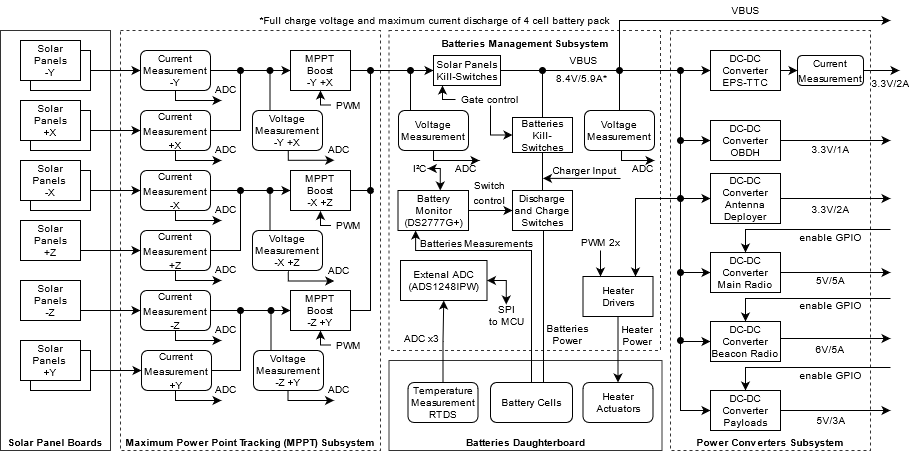
\includegraphics[width=\textwidth, keepaspectratio]{images/eps2-power-diagram.png}
    \end{center}
    \fonte{\textcite{eps2-doc}.}
    \label{fig:eps2-diagrama-blocos}
\end{figure}

Este módulo implementa uma topologia de distribuição centralizada, com múltiplos estágios de conversão, sistema de harvesting com \gls{PPT} e barramento principal não regulado.
Possui também um microcontrolador para operação, leitura de sensores e comunicação cos os demais módulos do satélite.

O sistema de harvesting consiste em três canais com conversores boost discretos e sensores de tensão e corrente, controlados individualmente pelo microcontrolador para realizar \gls{MPPT}, utilizando o algoritmo de \gls{PO}.

O sistema de distribuição consiste em seis barramentos com conversores dedicados, de 3.3V, 5V ou 6V, para cada um dos módulos do satélite, que podem ser ativados ou desativados individualmente.

O sistema de armazenamento consiste de um sistema de monitoramento (chamado \textit{Batteries Management Subsystem} na \autoref{fig:eps2-diagrama-blocos}) e de um módulo de baterias separado (chamado \textit{Batteries Daughterboard} no diagrama da \autoref{fig:eps2-diagrama-blocos}), que pode ser acoplado ao \gls{EPS2}.
O módulo de baterias contem 4 células de baterias de íon de lítio em configuração 2s-2p, bem como sensores de temperatura e aquecedores que podem ser lidos e controlados pelo microcontrolador do \gls{EPS}.
O sistema de monitoramento é realizado pelo CI DS2777G+, que realiza leituras de tensão e corrente das baterias, proteção contra over-charge e over-discharge, estimativas de vida útil e monitoramento do estado de carga das baterias.
Os sensores de temperatura são lidos por um conversor AD dedicado ADS1248 e utilizados para controle dos aquecedores de bateria, os driver para acionamento dos aquecedores, assim como o conversor AD,ficam no próprio \gls{EPS} e são controlados pelo microcontrolador.

O microcontrolador utilizado é um MSP430F6659 de 16 bits e de baixo consumo.
Suas principais funções são: leitura de sensores, comunicação com os demais módulos, monitoramento das baterias, controle dos aquecedores de bateria e execução do algoritmo para\gls{MPPT}.


%  ==== REEPS ====
\subsubsection{\texorpdfstring{RE\textsuperscript{2}PS}{REEPS}}


O \gls{REEPS} é um módulo de \gls{EPS} que está sendo desenvolvido pelo SpaceLab com o objetivo de atingir alta confiabilidade e robustez, tanto em termos de resistência à radiação quanto resistência a falhas.
No momento da escrita deste trabalho, o primeiro modelo de engenharia do \gls{REEPS} está em processo de fabricação.
Na \autoref{fig:reeps-diagrama-blocos} observa-se o diagrama de blocos deste sistema.

% Diagrama de blocos do REEPS
\begin{figure}[htp]
    \caption{Diagrama de blocos do RE\textsuperscript{2}PS}
    \begin{center}
        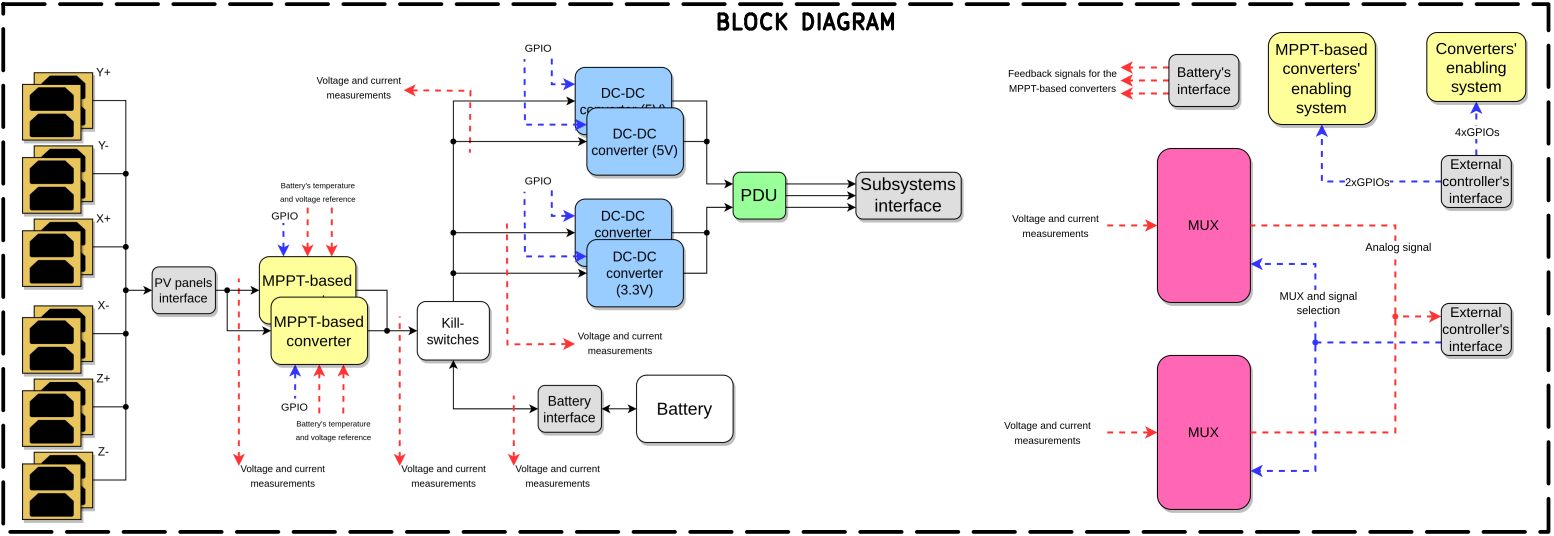
\includegraphics[width=\textwidth, keepaspectratio]{images/reeps-block-diagram.png}
    \end{center}
    \fonte{\textcite{reeps-doc}.}
    \label{fig:reeps-diagrama-blocos}
\end{figure}

Este módulo possui sistema de distribuição centralizado, sistema de harvesting com \gls{PPT}, múltiplos estágios de conversão e barramento principal não regulado.
Possui redundâncias em hardware nos principais subsistemas e não utiliza microcontrolador, visando aumentar a robustez à radiação.

O sistema de harvesting consiste em um barramento com dois \gls{BCR}s BQ24650, configurados em redundância fria, para realização de \gls{MPPT} e sensores de corrente e tensão na entrada e saída dos reguladores.

O sistema de armazenamento, similarmente ao \gls{EPS2}, utilizará um módulo de baterias dedicado, atualmente em estágio inicial de desenvolvimento.
\red{Confirmar!!}

O sistema de distribuição é composto por dois barramentos regulados, de 3.3V e 5V, seis canais de saída controlados individualmente e sensores de tensão e corrente em diversos pontos.
Cada barramento utiliza dois reguladores LTC3833 configurados em redundância fria e sensor de tensão à saída do regulador. Os canais de saída possui também sensores de corrente individuais para monitoramento.

Os sinais de todos os sensores podem ser acessados e lidos através de um multiplexador analógico presente no \gls{EPS}.



% ----------------------------------------------------------


% ----------------------------------------------------------
\section{Campanhas de teste de EPS}\label{sec:testes-epss}
% ----------------------------------------------------------

Além da arquitetura dos módulos, alguns dos trabalhos analisados apresentaram também os testes realizados em seus \gls{EPS}s, que serão apresentados a seguir.

\subsection{Aalto-2}

No trabalho de \textcite{aalto-eps}, é descrito o planejamento de testes para o EPS do satélite Aalto-2, assim como são relatados os resultados de testes executados em um modelo protótipo do mesmo.

O planejamento de testes descrito referenciou-se nas orientações do \gls{CDS} e suas filosofias de teste.
No momento da escrita do trabalho de \textcite{aalto-eps}, estavam previstos a fabricação de um modelo de engenharia para realização de testes funcionais e, posteriormente, a fabricação de um modelo de qualificação ou proto-flight para os testes de qualificação.

Os testes relatados no trabalho foram executados em um modelo protótipo nos estágios iniciais de desenvolvimento, sem o microcontrolador integrado ao módulo. Foram relatados os seguintes testes:

\begin{alineas}
    \item Funcionamento dos conversores DC-DC;
    \item Eficiência do sistema de harvesting (conversores \gls{BCR});
    \item Testes dos circuitos de proteção;
    \item Testes de burn-in;
\end{alineas} 

O funcionamento dos conversores DC-DC foi testado aplicando-se diferentes cargas (incrementalmente até atingirem-se os valores descritos nos requisitos do módulo) à saída e medindo-se tensões e correntes de entrada e saída a fim de obter-se a eficiência. Como os conversores possuem redundância, foram testados tanto individualmente quanto em funcionamento paralelo (redundância quente).
Os resultados foram então comparados com os requisitos e também com as informações disponíveis nos datasheets dos conversores, visto que são componentes \gls{COTS}.

O sistema de harvesting foi testado simulando-se o ponto de operação dos painéis solares com fontes de bancada e aplicando-se um reostato ao barramento das baterias. Foram medidas tensões e correntes à entrada e saída dos conversores \gls{BCR} utilizados para realizar \gls{MPPT} a fim de obter-se a eficiência.
Os resultados foram então comparados com os requisitos.

Para proteção contra over-current é utilizado o componente MAX890L. Sua operação foi testada aplicando-se passagem de corrente ao componente de forma incremental até que o limite imposto fosse atingido.

O teste de burn-in consistiu em aplicar uma alta demanda de potência ao EPS por um longo período de tempo.
Foram aplicadas cargas de 4.5W e 2.5W aos conversores de 5V e 3.3V, respectivamente, por um período de 7 dias. Após o teste, as características da placa foram medidas e comparadas com resultados anteriores.

\subsection{ESTCube-1}

No artigo de \textcite{estcube-eps} são relatados os testes realizados para qualificação do \gls{EPS} do satélite ESTCube-1. A filosofia de testes adotada foi de \textit{proto-flight testing}, ou seja, o mesmo módulo utilizado nos testes de qualificação foi utilizado como modelo de voo.
Um modelo de engenharia testes funcionais e de desenvolvimento, porém estes não foram descritos detalhadamente no artigo.

Foram relatados os seguintes testes:
\begin{alineas}
    \item Vibração senoidal e aleatória;
    \item Choque mecânico;
    \item Ciclagem térmica;
    \item Termo vácuo;
\end{alineas}

Além disso, foram realizados testes de estresse dos principais componentes do módulo antes da montagem do \gls{EPS}, incluindo testes de ciclagem térmica, ciclagem de carga e em vácuo das baterias utilizadas.

Foram medidas também a eficiência dos conversores utilizados, para diferentes tensões de entrada e diferentes cargas.


\subsection{MIST}

O trabalho de \textcite{mist-eps} descreve em detalhe os procedimentos de testes funcionais realizados no \gls{EPS} do satélite MIST.
Neste CubeSat, foram empregados módulos comerciais para toda a plataforma de serviço, inclusive para o \gls{EPS}, utilizando o modelo NanoPower P31u \cite{p31u-datasheet} em conjunto com a placa de baterias BP4 \cite{bp4-datasheet}, ambos fabricados pela GomSpace.

Os principais objetivos destes testes funcionais eram: verificar a análise de \textit{power budget}, medir o \gls{DoD} das baterias e verificar que a demanda de potência das cargas úteis não interfere no funcionamento do \gls{EPS}.

Para a execução dos testes, foi desenvolvida uma plataforma de testes constituída por uma plataforma flat-sat, simuladores de painéis solares e simuladores de consumo das cargas úteis, todos estes desenvolvidos por estudantes que haviam participado do projeto anteriormente.

O planejamento dos testes foi feito seguindo as orientações da \gls{ECSS} para testes \cite{ecss-e-st-10-03}.
Os testes foram divididos em blocos, sendo o primeiro bloco com testes funcionais e os outros cinco blocos com testes de missão, simulando o consumo e tempo de acionamento de diferentes cargas úteis do satélite de acordo com a operação esperada.

A seguir estão listados, resumidamente, os principais testes executados no \gls{EPS} do satélite MIST, assim como as medidas realizadas em cada teste:

\begin{alineas}
    \item Funcionais:
    \begin{alineas}
        \item Proteção de overcurrent dos barramentos;
        \item Proteção contra overcharge e over discharge das baterias;
    \end{alineas}
    \item Nenhuma payload ligada:
    \begin{alineas}
        \item Cenários de melhor e pior caso;
        \item Medidas de consumo do sistema, potência dos painéis, tensão e temperatura da bateria em cada cenário;
    \end{alineas}
    \item Combinações de payloads ligadas:
    \begin{alineas}
        \item Cenários de melhor e pior caso;
        \item Medida de tensão e temperatura da bateria;
        \item Medida da potência de saída dos barramentos;
    \end{alineas}
    \item Fast Charge/Discharge da bateria:
    \begin{alineas}
        \item Usado como referência do carregamento e descarregamento da bateria com as condições máximas suportadas pelo EPS;
        \item Não é um cenário esperado durante a operação;
        % \item Mediram apenas a variação da tensão nas baterias, não levaram em conta a corrente para o acumulo de carga mais preciso;
    \end{alineas}
\end{alineas}



\subsection{EPS 2.0}

Encontra-se na documentação do \gls{EPS2} \cite{eps2-doc} um capítulo descrevendo os procedimentos de teste a serem executados no módulo.
Tem-se também documentados relatórios de testes feitos em modelos de engenharia deste \gls{EPS}.

A documentação para a missão GOLDS-UFSC \cite{golds-ufsc-doc}, na qual será utilizado este \gls{EPS}, apresenta-se uma matriz de testes base a ser adaptada e executada para cada um dos módulos que compõem o satélite.
Para cada módulo, testes mais específicos poderão ser acrescentados à matriz base, que é mostrada na \autoref{tab:matriz-testes-golds}.
Os testes foram organizados em blocos, envolvendo uma série de inspeções, testes elétricos, funcionais.

\begin{table}[htp]
    \ABNTEXfontereduzida
    \centering
    \caption{Matriz de testes do EPS 2.0.}
    \begin{tabular}{l|p{90mm}|p{5mm}}
        \toprule[1.5pt]
        Tipo de Teste     & Sub Testes & ID \\
        \midrule
        A. Inspeção Visual     & 1. Verificação da qualidade da embalagem \newline 2. Qualidade da fabricação e montagem da placa \newline 3. Comparação com modelo 3D \newline 4. Marcadores de camada \newline 5. Rótulos (comparação com esquemático) \newline 6. Fotos de alta resolução para documentação & TA1 \newline TA2 \newline TA3 \newline TA4 \newline TA5 \newline TA6 \\
        \midrule
        B. Inspeção Mecânica   & 1. Dimensões da placa e posição das furações \newline 2. Pesagem da placa & TB1 \newline TB2 \\
        \midrule
        C. Inspeção de Integração    & 1. Verificar pinagem dos conectores \newline 2. Verificar posicionamento dos conectores & TC1 \newline TC2 \\
        \midrule
        D. Inspeção Elétrica   & 1. Curtos nas soldas \newline 2. Componentes faltantes \newline 3. Pinos levantados \newline 4. Qualidade das soldas \newline 5. Componentes trocados \newline 6. \textit{Partnumber} dos componentes & TD1 \newline TD2 \newline TD3 \newline TD4 \newline TD5 \newline TD6 \\
        \midrule
        E. Testes Elétricos    & 1. Teste de continuidade \newline 2. Procedimentos de alimentação \newline 3. Medida de potência média de entrada consumida \newline 4. Medida de potência média à saída \newline 5. Temperatura das trilhas de potência \newline 6. Integridade dos sinais & TE1 \newline TE2 \newline TE3 \newline TE4 \newline TE5 \newline TE6 \\
        \midrule
        F. Testes Funcionais   & 1. Executar código de teste simples \newline 2. Executar código do sistema \newline 3. Verificar \textit{flags} de auto-teste de hardware do sistema \newline 4. Monitorar comportamento dos LEDs \newline 5. Monitorar os \textit{logs} da porta serial de \textit{debug} & TF1 \newline TF2 \newline TF3 \newline TF4 \newline TF5 \\
         \midrule
        G. Testes de Módulo     & 1. Revisar comportamento operacional \newline 2. Revisar cumprimento de requisitos e funcionalidades \newline 3. Revisar configuração e protocolo dos barramentos de comunicação \newline 4. Revisar pacotes de dados, barramentos de potência e sinais de controle \newline 5. Revisar casos críticos e avaliar danos \newline 6. Executar testes de código automatizados \newline 7. Rodar códigos de teste do sistema \newline 8. Executar o código estável mais recente e revisar o comportamento & TG1 \newline TG2 \newline TG3 \newline \newline TG4 \newline \newline TG5 \newline TG6 \newline TG7 \newline TG8  \\
        \bottomrule[1.5pt]
    \end{tabular}
    \fonte{Adaptado de \textcite{golds-ufsc-doc}.}
    \label{tab:matriz-testes-golds}
\end{table}

As inspeções e testes descritos acima foram executados no modelo de engenharia do \gls{EPS2}, além disso, testes funcionais adicionais foram acrescentados e executados. Os resultados detalhados encontram-se no relatório presente nos Apêndices A e B da documentação do \gls{EPS2} \cite{eps2-doc}. Observando-se estes relatórios, identificam-se os seguintes testes:

\begin{alineas}
    \item Inspeções:
    \begin{alineas}
        \item Visual;
        \item Mecânica;
        \item Elétrica;
        \item De integração;
    \end{alineas}
    \item Testes elétricos:
    \begin{alineas}
        \item Teste dos conversores;
    \end{alineas}
    \item Testes funcionais:
    \begin{alineas}
        \item Gravação do firmware;
        \item Barramentos de comunicação;
        \item Leitura dos sensores;
        \item Funcionamento do monitor de baterias (DS2777G+);
        \item Controle dos aquecedores de bateria;
        \item Funcionamento do algoritmo de \gls{MPPT};
    \end{alineas}
\end{alineas}

Para todos os testes, o \gls{EPS} foi alimentado por uma fonte de bancada, através de uma flat sat.

As inspeções visam verificar a qualidade do processo de fabricação, conformidade com os arquivos de projeto e integridade mecânica e elétrica do módulo.

Os testes dos conversores foram realizados aplicando-se diferentes cargas à saída de cada barramento do \gls{EPS}, avaliando-se a ocorrência de quedas de tensão ou outras anomalias.

A versão mais recente do firmware foi gravada ao MSP430 e o funcionamento foi aferido através dos logs enviados ao computador via \gls{UART}.

Os principais barramentos de comunicação, com o \gls{OBDH} via \gls{I2C} e com o \gls{TTC} via \gls{UART}, foram testados utilizando-se um analisador lógico e verificando a integridade dos pacotes enviados.

A leitura dos sensores foi verificada comparando-se as medidas reportadas nos logs do \gls{EPS} com medidas realizadas por instrumentos de medição externos.

O funcionamento do monitor de baterias foi verificado através da leitura dos registradores internos do CI, comparando-se com os valores e configurações esperados.

Para o teste do controle dos aquecedores de bateria, seus limiares máximo e mínimo de temperatura foram alterados para valores acima da temperatura ambiente (32°C e 26°C, respectivamente), e as leituras dos sensores de temperatura foram monitoradas durante um período de tempo.

O algoritmo de \gls{PO} para o \gls{MPPT} foi testado com testes unitários no firmware.
O sinal de \gls{PWM} gerado pelo microcontrolador e utilizado para controle dos conversores boost que realizam o \gls{MPPT} foi avaliado utilizando-se um osciloscópio.
% ---

% ---
% Metodologia
% ---
% ----------------------------------------------------------
\chapter{Metodologia}
% ----------------------------------------------------------

Com o intuito de propor uma estrutura organizada e completa para o plano de testes, as normas e padrões da \gls{ECSS} serão tomados como referencial.
Será feita ua análise mais detalhada dos documentos referentes a testes \cite{ecss-e-st-10-03} e verificação \cite{ecss-e-st-10-02}, indentificando-se os aspectos principais e de maior relevância considerando o cenário de uma missão universitária.

A fim de propor uma matriz de testes base, adaptavel a diferentes módulos,as topologias e arquiteturas de \gls{EPS} apresentadas, bem como as campanhas de testes de missões prévias, serão analisadas e consideradas. Indentificando-se os diferente aspectos e funcionalidades, assim como os diferentes testes executados, blocos de testes mais completos poderão ser propostos.

A participação em projetos como FloripaSat-1, GOLDS-UFSC e Constelação Catarina, os anos de experiência no desenvolmento e testes de módulos \gls{EPS}, bem como o convívio diário com professores e colegas de laboratório no ambiente do SpaceLab agregam um conhecimento prévio significativo acerca dos aspectos e do cenário do desenvolvimento de missões espaciais universitárias.
As considerações e adaptações adotadas acerca da aplicabilidade de certos apsectos das normas são resultado destas experiências.
% ---

% ---
% Desenvolvimento
% ---
% ----------------------------------------------------------
\chapter{Desenvolvimento}
% ----------------------------------------------------------


Conforme \textcite{ecss-e-st-10-03}, o plano de testes é desenvolvido de acordo com o plano de verificação, que define quais dos requisitos relacionados ao produto serão testados.
A partir do plano de testes, documentos complementares são gerados, relacionados à especificação dos testes, procedimentos de teste e por fim relarórios de teste.
Nas normas, o termo produto se refere ao item ao qual o plano de testes se aplica.

Além dos conceitos apresentados na \autoref{sec:normas-ecss}, estas normas contem uma série de definições e requisistos relacionados aos testes, além de linhas de base de testes a serem adotadas.
Para sua utilização é feito um processo de adequação, também chamado de tailoring, para cada produto, no caso deste trabalho, o \gls{EPS}.

Este processo de adequação inicia-se a partir de definições iniciais acerca do tipo de produto a qual o plano se aplicará e do tipo de modelos a serem utilizados, para então adaptarem-se as linha de base de testes e elaborar o plano de testes.

\red{Comentar sobre requisitos relacionados à condições de teste, tolerancias, incertezas e etc. No caso, serão referenciadas diretamente as normas no documento como recomendações, visto que aplica-los à risca em uma missão universitária seria demasiado demorado e custoso (basicamente impossivel)}

O plano de testes base proposto neste trabalho consistirá de um documento contendo um conjunto de orientações e direcionamentos, detalhando os principais aspectos e considerações relevantes acerca da adaptação destas normas para módulos \gls{EPS} de forma que, a partir dele, possa-se elaborar planos de teste para diferentes topologias e arquiteturas de \gls{EPS}.

O documento proposto abordará os seguintes tópicos:
\begin{itemize}
    \item objetivo do plano de testes;
    \item blocos de testes;
    \item matriz de testes base;
    \item documentação.
\end{itemize}







% falar direto das definições relacionadas aos testes e linkar com verificação conforme mostrado na fundamentação, não explicar verificação primeiro para eventualmente chegar nos testes

% blocos de testes
% definição da matriz de testes

% intensidade e duração conforme objetivo, vide tabelas das normas


% The tailoring is applied in three steps:
% • First step: Tailoring is based upon the type of product and selected model philosophy. It consists of the selection of the relevant clauses as presented in Figure D-2.

% NOTE Should your model philosophy combine several models (e.g. QM+FM, or PFM+FM) the relevant clauses for both models need to be selected and merged when performing the second step.

% • Second step: The second tailoring consists in the consolidating Table 5-1, Table 5-3, Table 5-5, Table 6-1, Table 6-3 and Table 6-5 as they were selected in the First step.

% • Third step: The clause and Table called up on Table(s) consolidated at the Second step needs to be added, appropriately merged and tailored. At the end of the three steps, a new document is build which is the tailored Testing standard for a project application.

% The supplier responds to this document by a compliance matrix.

% When performing the three above steps the following points needs to be covered:

% • review the terms in clause 3 to ensure their proper use when performing the tailoring steps;

% • agree, as needed, on the nature of the item (space segment equipment versus space segment element) as per requirement 4.1b, and for equipment, agree the type of, or combination of types (as per Table 5-1 or Table 5-3 or Table 5-5);

% • agree on Test block definition as per requirement 4.3.2.1b in particular for equipment;

% • establish test matrix and test flow based on Figure 5-1 and Table 5-1 or Table 5-3 or Table 5-5 for equipment and Table 6-1, Table 6-3or Table 6-5for space segment element;

% • tailor the corresponding test level and duration based on corresponding Table 5-1 and Table 5-2 or Table 5-4 or Table 5-6 for equipment and Table 6-2, Table 6-4or Table 6-6for space segment element;

% • take the requirements of clauses 5.5 or 6.5 in accordance with the test table(s) (see column “Reference clause”) and tailor them;

% NOTE When several models are considered reference from various tables need to be considered taking into account the tailoring performed for each model.

% • include clause 4.6 in case of re-testing;

% • include clause 7 in case of PFM or FM stand-alone space segment element.


\red{
Tópicos importantes:
\begin{itemize}
    \item Considerações iniciais:
    \begin{itemize}
        \item Verification level.
        \item Verification stage.
        \item Model philosophy.
    \end{itemize}
    \item Estrutura do plano de testes.
    \begin{itemize}
        \item Blocos de teste.
        \item "Atividades" de teste.
        \item Estrutura da documentação.
    \end{itemize}
    \item Matriz de testes base da ECSS.
    \item Descrição de cada bloco de testes.
    \begin{itemize}
        \item Objetivo de cada bloco.
        \item Testes necessários em cada bloco para um EPS.
        \item Considerações adicionais.
    \end{itemize}
    \item Documentação.
\end{itemize}
}

% ----------------------------------------------------------
\section{Considerações Iniciais}
% ----------------------------------------------------------

De acordo com \textcite{ecss-e-st-10-02}, o processo de verificação é dividido em níveis de decomposição do sistema (\textit{verification levels}). Para cada nível, a verificação é feita multiplos estagíos (\textit{verification stages}), com objetivos específicos.
Testes se enquadram como um dos métodos utilizados dentro deste processo, inclusive sendo considerado o método que traz maior confiabilidade \cite{ecss-e-st-10-02}.

Desta forma, um plano de testes deve considerar o nível e estágio do processo de verificação no qual ele será executado.
Além disso, devem ser definidos os tipos de modelos físicos \textit{model philosophy} a serem utilizados nos testes.
O estágio de verificação, bem como o tipo de modelo adotado, definirão o objetivo principal do plano de testes elaborado.

A partir destas considerações, uma análise deve ser feita de modo que estes conceitos possam ser adaptados e aplicados a um módulo \gls{EPS} para CubeSats.


% ----------------------------------------------------------
\subsection{Nível de Verificação}
% ----------------------------------------------------------


O nível de verificação (\textit{verification level}) está relacionado com a decomposição do sistema em diferentes níveis nos quais o processo de verificação é executado.
Na tabela do apendice b.1 de ecss-s-st-00-01 mostra as divisoes típicas, com exemplos.

Em ecss-e-st-10-03, tratam-se dos testes para os níveis de \textit{space segment element} e \textit{space segment equipment}. O nível de \textit{space segment subsystem}, intermediário à estes, não é coberto nesta norma, de fato, é mencionado que para este nível, normalmete executam-se apenas testes funcionais.

Num primeiro momento, devido às nomenclaturas utilizadas e aos exemplos da tabela menciona, parece intuitivo atribuir os subsistemas de um CubeSat, e portanto o \gls{EPS}, ao nível de \textit{space segment subsystem}, porém uma análise mais minuciosa é necessária.

Primeiramente, visto que a plataforma de serviço é o pricipal foco de desenvolvimento do SpaceLab, é de grande interesse que sejam aplicados testes mais completos aos seus módulos, além de apenas testes funcionais básicos.
Alem disso, analisando as definições presentes nas próprias normas da \gls{ECSS}, pode-se fazer argumento para a aplicação dos testes voltados para \textit{space segment element} aos módulos de serviço de CubeSat, mais específicamente, neste trabalho, ao\gls{EPS}.

Como visto na \autoref{sec:cubesats}, os módulos de serviço são responsaveis pelas funções fundamentais do nano satélite, e estão diretamente relacionados com o cumprimento de seus objetivos.
Observando a defnição para o termo \textit{element}, nota-se que este está relacionado justamente com o cumprimento de um subconjunto dos objetivos do satélite.

\begin{citacao}
    element: combination of integrate equipment, components and parts. An element fulfils a major, self-contained, subset of a segment's objectives. \cite[p. 9]{ecss-s-st-00-01}.
\end{citacao}.

Além disso, nas próprias normas o termo \textit{service module} (módulo de serviço) é mencionado com \textit{element}. De fato, é mencionado tanto em \textcite{ecss-s-st-00-01} quanto em \textcite{ecss-e-st-10-03} que um elemento pode ser dividido em dois um mais elementos.

\begin{citacao}
    A space segment element cam be composed of several space segment elements, e.g. a spacecraft is composed of instruments, a payload module and a service module. \cite[p. 10]{ecss-s-st-00-01}
\end{citacao}.

Outro ponto importante, esta divisão proposta nas normas está no contexto de um satélite de médio ou grande porte, com sistemas de complexidade muito maiores que um CubeSat, portanto, uma decomposição mais granulada dos sistemas é adequada neste aspecto.
Mesmo neste cenário, em \textcite{ecss-e-hb-10-02}, é mencionado a possibilidade de não se utilizar o nível de subsistema como forma de redução de custos.

Com isto, neste trabalho serão consideradas as recomendações da norma ECSS-E-ST-10-03 \cite{ecss-e-st-10-03} relacionadas à \textit{space segment element}.

% \red{
%     Referencias para aplicar "element" ao EPS:
%     \begin{itemize}
%         \item ECSS-E-ST-10-03 Section 6.1a menciona dividir os testes de um "elemet" em service module tests e payload module tests;
%         \item Tabela do apendice B.1 de ECSS-S-ST-00-01 mostra module como "element" porém também mostra "power" como "subsystem";
%         \item Definições de "component", "equipment", "subsystem" e "element" em ECSS-S-ST-00-01 Section 2.2;
%         \item ECSS-S-ST-00-01 Section 2.2.4 menciona service module como "element";
%         \item ECSS-E-HB-10-02 Section 5.2.1.3.2 menciona descartar o nível de subsystem como redução de custos;
%     \end{itemize}
% Equipment executa uma função específica, subsystem executa um conjunto de funções, element satisfaz um subset dos objetivos de um segment
% }

% \red{Apresentar os demais níveis de decomposição? Talvez adicionar um parágrafo relacionado na \autoref{sec:normas-ecss}.}

% ----------------------------------------------------------
\subsection{Obejtivos do Plano de Testes}
% ----------------------------------------------------------

% Dentre os estágios de verificação apresentados na \autoref{sec:normas-ecss}, considerou-se \textit{qualification} e \textit{acceptance} como aplicáveis a nível de módulo, no contexto de um CubeSat.
% Estes estágios tem como finalidade qualificar o projeto do módulo e garantir seu funcionamento adequado e são fatores determinantes no objetivo do plano de testes.

% Após a execução destas estapas, o módulo estará apto a ser integrado ao restante do satélite, que passará por seu proprio processo de verificação a partir de então.


Considerando o estágio de verificação e tipo de modelo adotado, o plano de testes é definido com um dos três objetivos pricipais: \textit{qualification testing}, \textit{acceptance testing}, \textit{proto-flight testing}.
A descrição e finalidade de cada objetivo foi apresentada na \autoref{sec:normas-ecss}.

A principal consequencia de um determinado objetivo está na seleção dos testes a serem executados a partir das matrizes de teste base, e principalmente na intensidade e duração dos testes.

De fato, no documento ECSS-E-ST-10-03 \cite{ecss-e-st-10-03}, são apresentadas matrizes de teste base para cada objetivo de teste, sendo que a diferença entre cada uma está na definição de quais testes são considerados como requeridos ou opcionais.
Em relação à intensidade e duração dos testes, são apresentadas tabelas com os dados específicos para cada objetivo.

Em relação às intesidades e durações, serão referenciadas estas tabelas diretamente no plano de testes base quando necessário.






% ----------------------------------------------------------
\section{Linha de Base de Testes}
% ----------------------------------------------------------

As matrizes de testes base apresentadas em \textcite{ecss-e-st-10-03}, assim como o restante da norma, foram elaboradas de forma bastante abrangente e direcionadas à satélites de grande porte.
Sendo assim, considerando a simplicidade de projeto de um CubeSat e o contexto de uma missão universitária, uma versão bastante simplificada destas matrizes será adotada.

De fato, será porposta uma única matriz para os três diferentes objetivos, porém esta será elaborada de forma a abranger diferentes topologias e arquiteturas.
Ainda, visto que o plano de testes base é voltado diretamente para módulos \gls{EPS}, é possivel propor testes mais específicos, especialmente no caso de testes funcionais e de missão, proporcionando um maior direcionamento em relação as matrizes base.

% Considerações sobre testes em missões anteriores

Com isso, a partir das matrizes de testes base apresentadas na norma ECSS-E-ST-10-03 \cite{ecss-e-st-10-03}, consideraram-se os seguintes testes:

\begin{itemize}
    \item Funcionais;
    \item Performance;
    \item Missão;
    \item Propriedades físicas;
    \item Vibração;
    \item Termo vácuo.
    \item \red{EMC?}
\end{itemize}


Considerações a respeito de cada item


% ----------------------------------------------------------
\section{Testes Funcionais e de Performance}
% ----------------------------------------------------------

Incluir testes de missão aqui?

Selecionar testes funcionais consideranto as diferentes topologias e arquiteturas apresentadas


% ----------------------------------------------------------
\section{Matriz de Testes Base}
% ----------------------------------------------------------

Blocos de teste

Matriz proposta

Considerações a cerca da adaptação da matriz

% ----------------------------------------------------------
\section{Requisitos Adicionais}
% ----------------------------------------------------------

condições de teste, tolerância, incerteazs

Equipamentos utilizados e local de testes


% ----------------------------------------------------------
\section{Documentação}
% ----------------------------------------------------------

Apresentar estrutura do documento de plano de testes, test specifications, procedures e report

% ---

% ---
% Resultados
% ---
% ----------------------------------------------------------
\chapter{Documento de Diretrizes}
% ----------------------------------------------------------

Com base nos estudos e analises realizadas, foi elaborado um documento, nomeado \textit{EPS Test Plan Guidelines} contendo diretrizes e recomendações acerca da elaboração de planos de teste para módulos \gls{EPS} no contexto de missões de CubeSats.

Visto que a utilização primária será para os módulos desenvolvidos no SpaceLab, e também motivação da realização do trabalho veio das experiências adquiridas na participação dos projetos do laboratório, foi utilizado o modelo e estilo de documentação utilizados no SpaceLab, no idioma Inglês.
No \autoref{app:plano-testes-base} pode ser encontrada a primeira versão deste documento.

O documento cobre os tópicos discutidos no \autoref{cap:desenvolvimento}, e está organizado da seguinte maneira:

\begin{alineas}
    \item introdução:
    \begin{alineas}
        \item contendo uma descrição do propósito do documento;
    \end{alineas}

    \item documentação:
    \begin{alineas}
        \item contendo uma estrutura base para o plano de testes, bem como uma descrição da documentação associada ao plano;
    \end{alineas}

    \item objetivos de teste:
    \begin{alineas}
        \item contendo uma descrição dos principais objetivos de um plano de testes.
    \end{alineas}

    \item requisitos gerais:
    \begin{alineas}
        \item contendo referência aos requisitos gerais de teste definidos nas normas;
    \end{alineas}

    \item matriz de testes base:
    \begin{alineas}
        \item contendo a matriz de testes base proposta, bem como uma descrição dos principais blocos e atividades de teste.
    \end{alineas}

\end{alineas}


Apesar de que a aplicação primária será aos módulos \gls{EPS} do SpaceLab, o documento foi elaborado de forma que possa ser utilizado por outros grupos, e para diferentes módulos \gls{EPS}, e estará em constante desenvolvimento e aprimoramento.
% ---

% ---
% Estudo de Caso
% ---
% ----------------------------------------------------------
\chapter{Estudo de Caso - EPS 2.0}
% ----------------------------------------------------------

A partir das diretrizes e orientações do documento \textit{EPS Test Plan Guidelines}, um plano de testes para o módulo \gls{EPS2}, desenvolvido no SpaceLab, foi elaborado.
No \autoref{app:plano-testes-eps2} pode ser encontrada a primeira versão deste documento.

O testes foram selecionados considerando a execução nas instalações do SpaceLab, levando em conta os equipamentos e infraestrutura disponíveis no mesmo. Por este motivo, testes ambientais não foram incluídos.

Ainda, visto que um dos interesses do laboratório é de viabilizar a comparação de performance entre os diferentes módulos de \gls{EPS} desenvolvidos, um requisito adicional representando este propósito, foi adicionado ao plano, além dos requisitos da missão deste módulo.

O documento foi estruturado da seguinte maneira:


\begin{alineas}
    \item introdução:
    \begin{alineas}
        \item contendo uma descrição do propósito do plano de testes, bem como considerações acerca de sua elaboração;
    \end{alineas}

    \item modelos de hardware:
    \begin{alineas}
        \item contendo uma descrição dos modelos físicos a serem utilizados para os testes e seu estado de construção;
    \end{alineas}

    \item requisitos a serem verificados:
    \begin{alineas}
        \item contendo uma listagem dos requisitos da missão verificados por este plano de testes.
    \end{alineas}

    \item programa de testes:
    \begin{alineas}
        \item contendo a matriz de testes proposta, descrição dos principais blocos e atividades de teste e fluxo de execução.
    \end{alineas}

    \item instalações de teste:
    \begin{alineas}
        \item contendo uma descrição das instalações a serem utilizadas e listagem dos equipamentos disponíveis;
    \end{alineas}

    \item documentação:
    \begin{alineas}
        \item contendo uma descrição dos documentos a serem elaborados a partir deste plano de testes;
    \end{alineas}

\end{alineas}
% ---

% ---
% Conclusão
% ---
%\phantompart
% ----------------------------------------------------------
\chapter{Conclusão}
% ----------------------------------------------------------

As conclusões devem responder às questões da pesquisa, em relação aos objetivos e às hipóteses. Devem ser breves, podendo apresentar recomendações e sugestões para trabalhos futuros.
% ---

% ----------------------------------------------------------
% ELEMENTOS PÓS-TEXTUAIS
% ----------------------------------------------------------
\postextual
% ----------------------------------------------------------

% ----------------------------------------------------------
% Referências bibliográficas
% ----------------------------------------------------------
\begingroup
    \SingleSpacing\printbibliography[title=REFERÊNCIAS]
\endgroup

% ----------------------------------------------------------
% Glossário
% ----------------------------------------------------------
%
% Consulte o manual da classe abntex2 para orientações sobre o glossário.
%
%\glossary

% ----------------------------------------------------------
% Apêndices
% ----------------------------------------------------------

% ---
% Inicia os apêndices
% ---
\begin{apendicesenv}
%	\partapendices* 
	% % ----------------------------------------------------------
\chapter{Descrição}
% ----------------------------------------------------------

Textos elaborados pelo autor, a fim de completar a sua argumentação. Deve ser precedido da palavra APÊNDICE, identificada por letras maiúsculas consecutivas, travessão e pelo respectivo título. Utilizam-se letras maiúsculas dobradas quando esgotadas as letras do alfabeto. 

\begin{quadro}[htb]
	\centering
	\caption{\label{qua:Quadro_2}Modelo A.}	
\begin{tabular}{|l|l|}
\hline
xxxx              & yyyyyyyyyyyyyyy    \\
\hline
xxxx              & yyyyyyyyyyyyyyy    \\
\hline
xxxx              & yyyyyyyyyyyyyyy    \\
\hline
xxxx              & yyyyyyyyyyyyyyy    \\
\hline
xxxx              & yyyyyyyyyyyyyyy    \\
\hline
xxxx              & yyyyyyyyyyyyyyy    \\
\hline
xxxx              & yyyyyyyyyyyyyyy    \\
\hline
rrrrrrrrrrrrrrrrr & eeeeeeeeeeeeeeeee  \\
\hline
xxxx              & yyyyyyyyyyyyyyy    \\
\hline
xxxx              & yyyyyyyyyyyyyyy    \\
\hline
rrrrrrrrrrrrrrrrr & eeeeeeeeeeeeeeeee  \\
\hline
xxxx              & yyyyyyyyyyyyyyy    \\
\hline
                  & ttttttttttttttttt  \\
\hline
rrrrrrrrrrrrrrrrr & eeeeeeeeeeeeeeeee  \\
\hline
ttttttttttttt     &                    \\
\hline
rrrrrrrrrrrrrrrrr & eeeeeeeeeeeeeeeee  \\
\hline
rrrrrrrrrrrrrrrrr & eeeeeeeeeeeeeeeee  \\
\hline
                  & gggggggggggggggggg \\
\hline
rrrrrrrrrrrrrrrrr & eeeeeeeeeeeeeeeee  \\
\hline
rrrrrrrrrrrrrrrrr & eeeeeeeeeeeeeeeee  \\
\hline
rrrrrrrrrrrrrrrrr & eeeeeeeeeeeeeeeee  \\
\hline
rrrrrrrrrrrrrrrrr & eeeeeeeeeeeeeeeee  \\
\hline
\end{tabular}
\fonte{Elaborada pelo autor (2016).}
\end{quadro}

	% ----------------------------------------------------------
\chapter{Documento de Diretrizes} \label{app:plano-testes-base}
% ----------------------------------------------------------

A seguir é apresentada a primeira versão do documento de diretrizes desenvolvido neste trabalho.


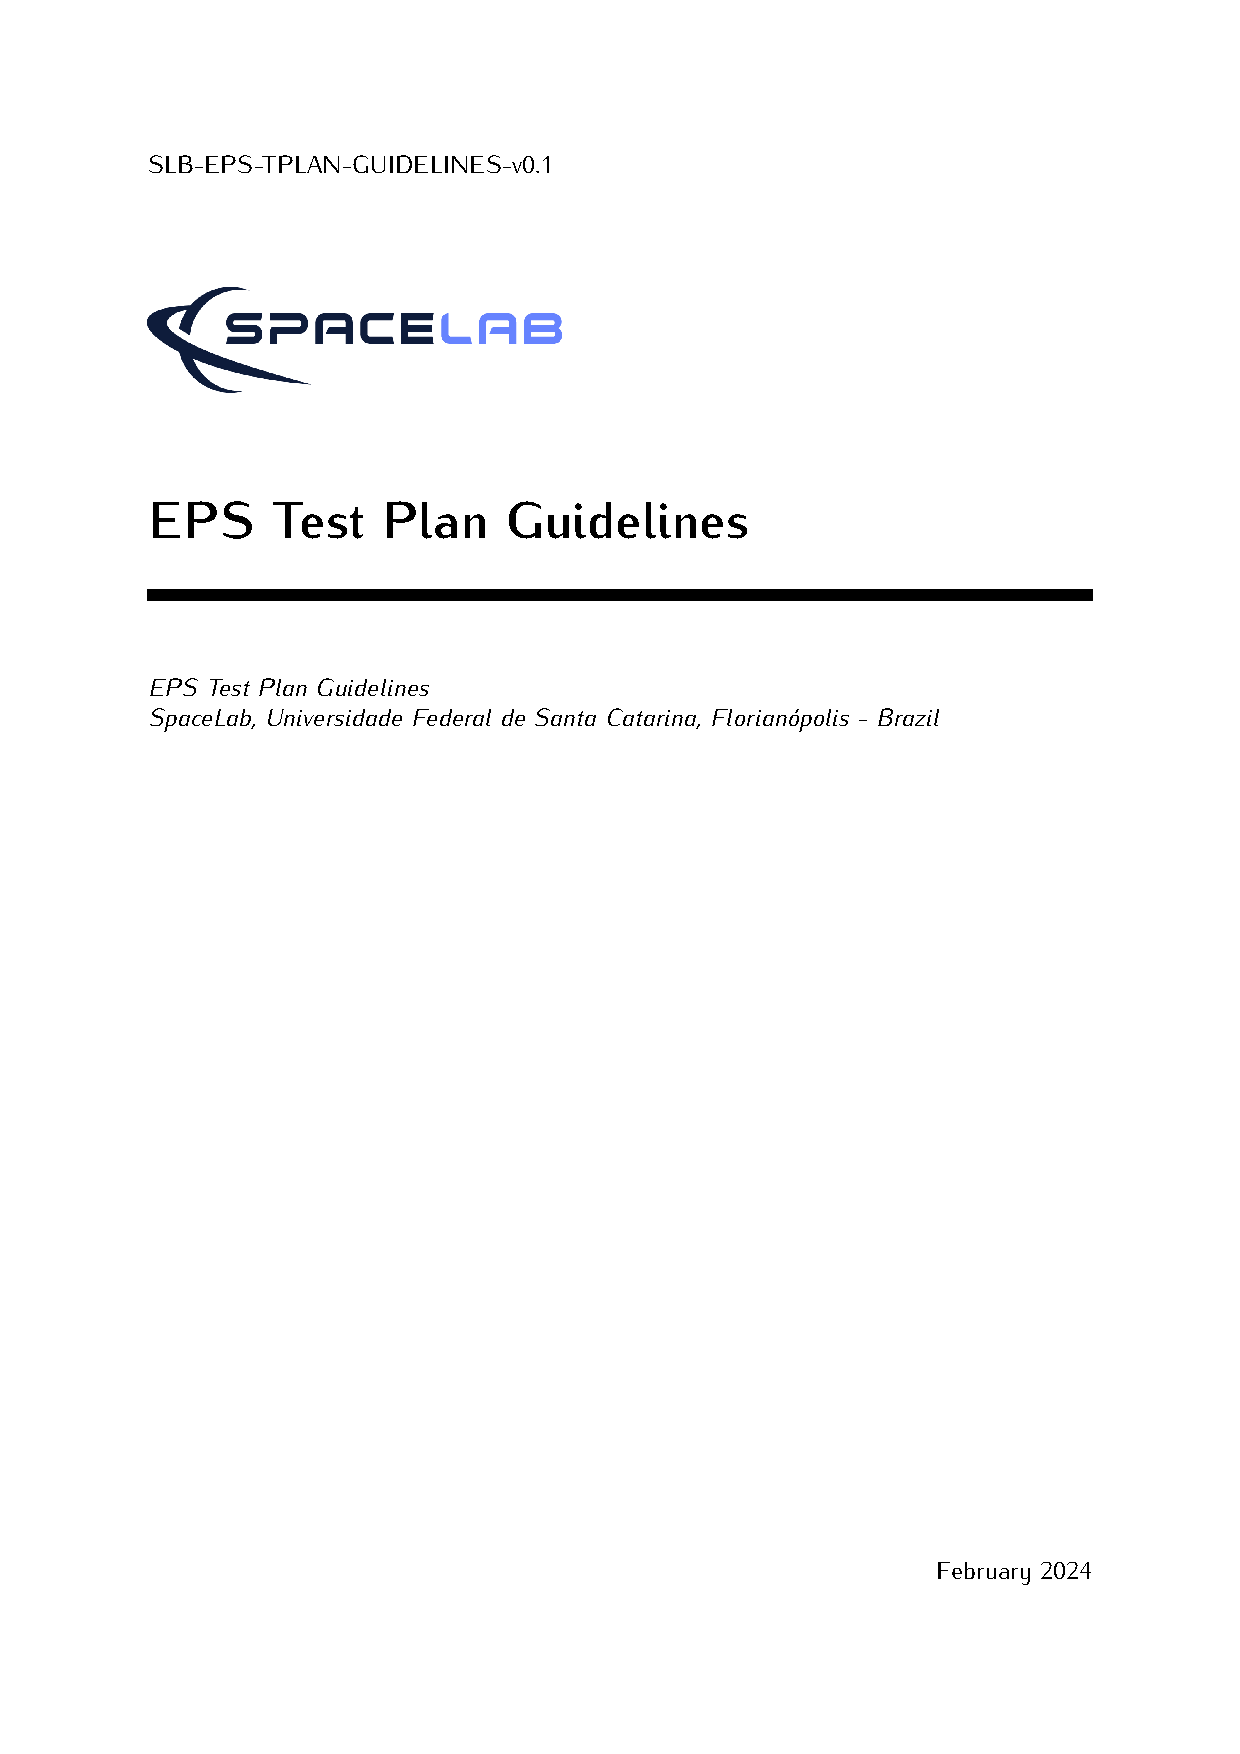
\includepdf[scale=1, pages=-, pagecommand={}]{documents/slb-eps-tplan-guidelines-v0.1.pdf}



	% ----------------------------------------------------------
\chapter{Plano de Testes EPS 2.0}
% ----------------------------------------------------------

A seguir é apresentada a primeira versão do plano de testes desenvolvido para o módulo \gls{EPS2} desenvolvido pelo SpaceLab.



\includepdf[scale=1,pages=-,pagecommand={}]{documents/slb-eps2-ql-tplan-v0.1.pdf}


\end{apendicesenv}
% ---


% ----------------------------------------------------------
% Anexos
% ----------------------------------------------------------

% ---
% Inicia os anexos
% % ---
% \begin{anexosenv}
% %	\partanexos*
% 	% ----------------------------------------------------------
\chapter{Descrição}
% ----------------------------------------------------------

São documentos não elaborados pelo autor que servem como fundamentação (mapas, leis, estatutos). Deve ser precedido da palavra ANEXO, identificada por letras maiúsculas consecutivas, travessão e pelo respectivo título. Utilizam-se letras maiúsculas dobradas quando esgotadas as letras do alfabeto. 

% \end{anexosenv}

%---------------------------------------------------------------------
% INDICE REMISSIVO
%---------------------------------------------------------------------
%\phantompart
%\printindex
%---------------------------------------------------------------------

\end{document}
